\documentclass[a4paper]{book}
\usepackage{a4wide}
\usepackage{makeidx}
\usepackage{fancyhdr}
\usepackage{graphicx}
\usepackage{multicol}
\usepackage{float}
\usepackage{textcomp}
\usepackage{alltt}
\usepackage{times}
\usepackage{ifpdf}
\ifpdf
\usepackage[pdftex,
            pagebackref=true,
            colorlinks=true,
            linkcolor=blue,
            unicode
           ]{hyperref}
\else
\usepackage[ps2pdf,
            pagebackref=true,
            colorlinks=true,
            linkcolor=blue,
            unicode
           ]{hyperref}
\usepackage{pspicture}
\fi
\usepackage[utf8]{inputenc}
\usepackage{doxygen}
\makeindex
\setcounter{tocdepth}{1}
\renewcommand{\footrulewidth}{0.4pt}
\begin{document}
\begin{titlepage}
\vspace*{7cm}
\begin{center}
{\Large beam\_\-dump Reference Manual\\[1ex]\large 0.1 }\\
\vspace*{1cm}
{\large Generated by Doxygen 1.5.3}\\
\vspace*{0.5cm}
{\small Thu Sep 25 17:52:06 2008}\\
\end{center}
\end{titlepage}
\clearemptydoublepage
\pagenumbering{roman}
\tableofcontents
\clearemptydoublepage
\pagenumbering{arabic}
\chapter{beam\_\-dump Hierarchical Index}
\section{Class Hierarchy}
This inheritance list is sorted roughly, but not completely, alphabetically\-:\begin{DoxyCompactList}
\item \contentsline{section}{Element}{\pageref{classElement}}{}
\item \contentsline{section}{Geometry}{\pageref{classGeometry}}{}
\begin{DoxyCompactList}
\item \contentsline{section}{Cone}{\pageref{classCone}}{}
\begin{DoxyCompactList}
\item \contentsline{section}{Cone2}{\pageref{classCone2}}{}
\end{DoxyCompactList}
\item \contentsline{section}{Cone2}{\pageref{classCone2}}{}
\item \contentsline{section}{Cylinder}{\pageref{classCylinder}}{}
\item \contentsline{section}{Ogive}{\pageref{classOgive}}{}
\item \contentsline{section}{Ring}{\pageref{classRing}}{}
\item \contentsline{section}{Two\-Plates}{\pageref{classTwoPlates}}{}
\end{DoxyCompactList}
\item \contentsline{section}{Node}{\pageref{classNode}}{}
\item \contentsline{section}{Particle}{\pageref{classParticle}}{}
\item \contentsline{section}{Simulation}{\pageref{classSimulation}}{}
\end{DoxyCompactList}

\chapter{beam\_\-dump Class Index}
\section{Class List}
Here are the classes, structs, unions and interfaces with brief descriptions\-:\begin{DoxyCompactList}
\item\contentsline{section}{\hyperlink{classCone}{Cone} }{\pageref{classCone}}{}
\item\contentsline{section}{\hyperlink{classCone2}{Cone2} }{\pageref{classCone2}}{}
\item\contentsline{section}{\hyperlink{classCylinder}{Cylinder} }{\pageref{classCylinder}}{}
\item\contentsline{section}{\hyperlink{classElement}{Element} }{\pageref{classElement}}{}
\item\contentsline{section}{\hyperlink{classGeometry}{Geometry} }{\pageref{classGeometry}}{}
\item\contentsline{section}{\hyperlink{classNode}{Node} }{\pageref{classNode}}{}
\item\contentsline{section}{\hyperlink{classOgive}{Ogive} }{\pageref{classOgive}}{}
\item\contentsline{section}{\hyperlink{classParticle}{Particle} }{\pageref{classParticle}}{}
\item\contentsline{section}{\hyperlink{classRing}{Ring} }{\pageref{classRing}}{}
\item\contentsline{section}{\hyperlink{classSimulation}{Simulation} }{\pageref{classSimulation}}{}
\item\contentsline{section}{\hyperlink{classTwoPlates}{Two\-Plates} }{\pageref{classTwoPlates}}{}
\end{DoxyCompactList}

\chapter{beam\_\-dump File Index}
\section{File List}
Here is a list of all files with brief descriptions\-:\begin{DoxyCompactList}
\item\contentsline{section}{src/\hyperlink{cone_8cpp}{cone.\-cpp} }{\pageref{cone_8cpp}}{}
\item\contentsline{section}{src/\hyperlink{cone_8h}{cone.\-h} \\*Pure conical geometry }{\pageref{cone_8h}}{}
\item\contentsline{section}{src/\hyperlink{cone2-bak_8cpp}{cone2-\/bak.\-cpp} }{\pageref{cone2-bak_8cpp}}{}
\item\contentsline{section}{src/\hyperlink{cone2-bak_8h}{cone2-\/bak.\-h} }{\pageref{cone2-bak_8h}}{}
\item\contentsline{section}{src/\hyperlink{cone2_8cpp}{cone2.\-cpp} }{\pageref{cone2_8cpp}}{}
\item\contentsline{section}{src/\hyperlink{cone2_8h}{cone2.\-h} }{\pageref{cone2_8h}}{}
\item\contentsline{section}{src/\hyperlink{cylinder_8cpp}{cylinder.\-cpp} }{\pageref{cylinder_8cpp}}{}
\item\contentsline{section}{src/\hyperlink{cylinder_8h}{cylinder.\-h} \\*Pure cylindrical geometry }{\pageref{cylinder_8h}}{}
\item\contentsline{section}{src/\hyperlink{element_8cpp}{element.\-cpp} }{\pageref{element_8cpp}}{}
\item\contentsline{section}{src/\hyperlink{element_8h}{element.\-h} \\*Facet planar geometry for graphical representation purposes }{\pageref{element_8h}}{}
\item\contentsline{section}{src/\hyperlink{geometry_8cpp}{geometry.\-cpp} }{\pageref{geometry_8cpp}}{}
\item\contentsline{section}{src/\hyperlink{geometry_8h}{geometry.\-h} \\*Base class for the different geometries }{\pageref{geometry_8h}}{}
\item\contentsline{section}{src/\hyperlink{heatsurf_8cpp}{heatsurf.\-cpp} }{\pageref{heatsurf_8cpp}}{}
\item\contentsline{section}{src/\hyperlink{node_8cpp}{node.\-cpp} }{\pageref{node_8cpp}}{}
\item\contentsline{section}{src/\hyperlink{node_8h}{node.\-h} \\*\hyperlink{classNode}{Node} class for graphical representation purposes }{\pageref{node_8h}}{}
\item\contentsline{section}{src/\hyperlink{ogive_8cpp}{ogive.\-cpp} }{\pageref{ogive_8cpp}}{}
\item\contentsline{section}{src/\hyperlink{ogive_8h}{ogive.\-h} }{\pageref{ogive_8h}}{}
\item\contentsline{section}{src/\hyperlink{particle_8cpp}{particle.\-cpp} }{\pageref{particle_8cpp}}{}
\item\contentsline{section}{src/\hyperlink{particle_8h}{particle.\-h} \\*Represents each of the finite charged particles }{\pageref{particle_8h}}{}
\item\contentsline{section}{src/\hyperlink{ring_8cpp}{ring.\-cpp} }{\pageref{ring_8cpp}}{}
\item\contentsline{section}{src/\hyperlink{ring_8h}{ring.\-h} \\*Anular geometry }{\pageref{ring_8h}}{}
\item\contentsline{section}{src/\hyperlink{simulation_8cpp}{simulation.\-cpp} }{\pageref{simulation_8cpp}}{}
\item\contentsline{section}{src/\hyperlink{simulation_8h}{simulation.\-h} \\*Procedures for the program workflow }{\pageref{simulation_8h}}{}
\item\contentsline{section}{src/\hyperlink{twoplates_8cpp}{twoplates.\-cpp} }{\pageref{twoplates_8cpp}}{}
\item\contentsline{section}{src/\hyperlink{twoplates_8h}{twoplates.\-h} \\*Two symmetrical plates geometry }{\pageref{twoplates_8h}}{}
\end{DoxyCompactList}

\chapter{beam\_\-dump Class Documentation}
\hypertarget{classCone}{
\section{Cone Class Reference}
\label{classCone}\index{Cone@{Cone}}
}
{\tt \#include $<$/home/dani/Programs/beam\_\-dump/src/cone.h$>$}

Inheritance diagram for Cone:\nopagebreak
\begin{figure}[H]
\begin{center}
\leavevmode
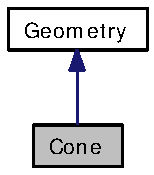
\includegraphics[width=55pt]{classCone__inherit__graph}
\end{center}
\end{figure}
Collaboration diagram for Cone:\nopagebreak
\begin{figure}[H]
\begin{center}
\leavevmode
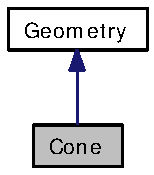
\includegraphics[width=55pt]{classCone__coll__graph}
\end{center}
\end{figure}
\subsection*{Public Member Functions}
\begin{CompactItemize}
\item 
\hypertarget{classCone_da9d6b717b3e91609b2500eba83e3c21}{
\textbf{Cone} (std::string, double, double, int)}
\label{classCone_da9d6b717b3e91609b2500eba83e3c21}

\item 
\hypertarget{classCone_984487f56d87dfa483c5bb957ae24eb3}{
void \textbf{computeEnergy} (double, std::vector$<$ \hyperlink{classParticle}{Particle} $\ast$ $>$ \&)}
\label{classCone_984487f56d87dfa483c5bb957ae24eb3}

\item 
\hypertarget{classCone_52fd80b6c484449a8d24d1471e21873c}{
void \textbf{setSections} (double)}
\label{classCone_52fd80b6c484449a8d24d1471e21873c}

\item 
\hypertarget{classCone_98c5dc0bc0561ab92e76a8ab4da2f891}{
void \textbf{computeGeometry} ()}
\label{classCone_98c5dc0bc0561ab92e76a8ab4da2f891}

\item 
\hypertarget{classCone_a026083e1c8ecfd1f589eb1939b302c1}{
void \textbf{outputTable} ()}
\label{classCone_a026083e1c8ecfd1f589eb1939b302c1}

\item 
\hypertarget{classCone_1df030d3ae438a08c7b34bbb63382e04}{
void \textbf{outputEnergyFile} ()}
\label{classCone_1df030d3ae438a08c7b34bbb63382e04}

\item 
\hypertarget{classCone_d80275cb6371a959b037e93ec2ad5bdf}{
void \textbf{outputPowerFile} ()}
\label{classCone_d80275cb6371a959b037e93ec2ad5bdf}

\end{CompactItemize}


\subsection{Detailed Description}
\begin{Desc}
\item[Author:]Daniel Iglesias $<$\href{mailto:daniel.iglesias@ciemat.es}{\tt daniel.iglesias@ciemat.es}$>$ \end{Desc}


The documentation for this class was generated from the following files:\begin{CompactItemize}
\item 
src/\hyperlink{cone_8h}{cone.h}\item 
src/cone.cpp\end{CompactItemize}

\hypertarget{classCylinder}{\section{Cylinder Class Reference}
\label{classCylinder}\index{Cylinder@{Cylinder}}
}


{\ttfamily \#include $<$/home/daniel.\-iglesias/\-Projects/\-Heat\-Surf/src/cylinder.\-h$>$}



Inheritance diagram for Cylinder\-:\nopagebreak
\begin{figure}[H]
\begin{center}
\leavevmode
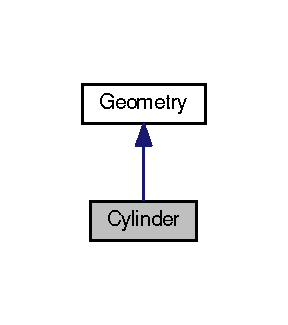
\includegraphics[width=138pt]{classCylinder__inherit__graph}
\end{center}
\end{figure}


Collaboration diagram for Cylinder\-:\nopagebreak
\begin{figure}[H]
\begin{center}
\leavevmode
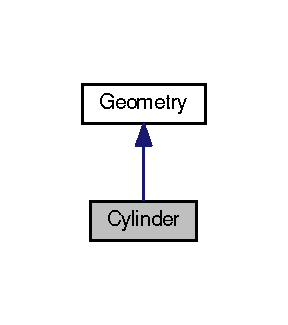
\includegraphics[width=138pt]{classCylinder__coll__graph}
\end{center}
\end{figure}
\subsection*{Public Member Functions}
\begin{DoxyCompactItemize}
\item 
\hyperlink{classCylinder_a01dc978cb576f834b9545e43d4dad2a2}{Cylinder} ()
\item 
\hyperlink{classCylinder_af6f22d1e11f65fc230f270c16e25385a}{Cylinder} (std\-::string, double, double, double, int)
\item 
\hyperlink{classCylinder_a05ab556f0ae3cd6e99d9d1f3caca80b3}{$\sim$\-Cylinder} ()
\item 
void \hyperlink{classCylinder_ad75a4b81272ef8b27b3163bf0aa49efd}{set\-Sections} (double)
\item 
void \hyperlink{classCylinder_a657d003c8da54cb8d5cf78bbe210cafa}{compute\-Geometry} ()
\item 
void \hyperlink{classCylinder_a76a83ba9168f8a9bc30bf0a85250f984}{residue} (lmx\-::\-Vector$<$ double $>$ \&, lmx\-::\-Vector$<$ double $>$ \&)
\item 
void \hyperlink{classCylinder_a27c6e57d5f10da5fc660adf731960d6f}{jacobian} (lmx\-::\-Matrix$<$ double $>$ \&, lmx\-::\-Vector$<$ double $>$ \&)
\item 
void \hyperlink{classCylinder_a3785595915b105f5e387a4b76d0d6ee9}{compute\-Intersection} (\hyperlink{classParticle}{Particle} $\ast$)
\item 
void \hyperlink{classCylinder_a950b48028c934fa9f01cb3ae40422aef}{compute\-Nodal\-Power} (\hyperlink{classParticle}{Particle} $\ast$)
\item 
void \hyperlink{classCylinder_a33abcb99e6c881b867a0bb6c0dfcabae}{output\-Table} ()
\item 
void \hyperlink{classCylinder_ab2481ec0318f4686fd7787696230b4bd}{output\-Power\-File} (int)
\item 
void \hyperlink{classCylinder_a82078ecb74fbe07bed3de4040be73125}{output\-Power\-Density\-File} ()
\end{DoxyCompactItemize}
\subsection*{Additional Inherited Members}


\subsection{Detailed Description}
\begin{DoxyAuthor}{Author}
Daniel Iglesias \href{mailto:daniel.iglesias@ciemat.es}{\tt daniel.\-iglesias@ciemat.\-es} 
\end{DoxyAuthor}


\subsection{Constructor \& Destructor Documentation}
\hypertarget{classCylinder_a01dc978cb576f834b9545e43d4dad2a2}{\index{Cylinder@{Cylinder}!Cylinder@{Cylinder}}
\index{Cylinder@{Cylinder}!Cylinder@{Cylinder}}
\subsubsection[{Cylinder}]{\setlength{\rightskip}{0pt plus 5cm}Cylinder\-::\-Cylinder (
\begin{DoxyParamCaption}
{}
\end{DoxyParamCaption}
)}}\label{classCylinder_a01dc978cb576f834b9545e43d4dad2a2}
\hypertarget{classCylinder_af6f22d1e11f65fc230f270c16e25385a}{\index{Cylinder@{Cylinder}!Cylinder@{Cylinder}}
\index{Cylinder@{Cylinder}!Cylinder@{Cylinder}}
\subsubsection[{Cylinder}]{\setlength{\rightskip}{0pt plus 5cm}Cylinder\-::\-Cylinder (
\begin{DoxyParamCaption}
\item[{std\-::string}]{type\-\_\-in, }
\item[{double}]{par0\-\_\-in, }
\item[{double}]{par1\-\_\-in, }
\item[{double}]{par2\-\_\-in, }
\item[{int}]{par3\-\_\-in}
\end{DoxyParamCaption}
)}}\label{classCylinder_af6f22d1e11f65fc230f270c16e25385a}


References Geometry\-::grid\-Width.

\hypertarget{classCylinder_a05ab556f0ae3cd6e99d9d1f3caca80b3}{\index{Cylinder@{Cylinder}!$\sim$\-Cylinder@{$\sim$\-Cylinder}}
\index{$\sim$\-Cylinder@{$\sim$\-Cylinder}!Cylinder@{Cylinder}}
\subsubsection[{$\sim$\-Cylinder}]{\setlength{\rightskip}{0pt plus 5cm}Cylinder\-::$\sim$\-Cylinder (
\begin{DoxyParamCaption}
{}
\end{DoxyParamCaption}
)}}\label{classCylinder_a05ab556f0ae3cd6e99d9d1f3caca80b3}


\subsection{Member Function Documentation}
\hypertarget{classCylinder_a657d003c8da54cb8d5cf78bbe210cafa}{\index{Cylinder@{Cylinder}!compute\-Geometry@{compute\-Geometry}}
\index{compute\-Geometry@{compute\-Geometry}!Cylinder@{Cylinder}}
\subsubsection[{compute\-Geometry}]{\setlength{\rightskip}{0pt plus 5cm}void Cylinder\-::compute\-Geometry (
\begin{DoxyParamCaption}
{}
\end{DoxyParamCaption}
)\hspace{0.3cm}{\ttfamily [virtual]}}}\label{classCylinder_a657d003c8da54cb8d5cf78bbe210cafa}


Implements \hyperlink{classGeometry_a3e77ac889d1e440c24efbde630aa1933}{Geometry}.



References Geometry\-::elements, Geometry\-::grid, Geometry\-::grid\-Points, Geometry\-::length, Geometry\-::nodes, Geometry\-::sections, Geometry\-::sectors, and Geometry\-::z0.

\hypertarget{classCylinder_a3785595915b105f5e387a4b76d0d6ee9}{\index{Cylinder@{Cylinder}!compute\-Intersection@{compute\-Intersection}}
\index{compute\-Intersection@{compute\-Intersection}!Cylinder@{Cylinder}}
\subsubsection[{compute\-Intersection}]{\setlength{\rightskip}{0pt plus 5cm}void Cylinder\-::compute\-Intersection (
\begin{DoxyParamCaption}
\item[{{\bf Particle} $\ast$}]{particle}
\end{DoxyParamCaption}
)\hspace{0.3cm}{\ttfamily [virtual]}}}\label{classCylinder_a3785595915b105f5e387a4b76d0d6ee9}


Implements \hyperlink{classGeometry_ac2e6c74ef25ff3e0c4f46b2c80484881}{Geometry}.



References Particle\-::get\-X(), Particle\-::get\-Xdiv(), Particle\-::get\-Y(), Particle\-::get\-Ydiv(), Particle\-::get\-Z(), Particle\-::get\-Zdiv(), jacobian(), Geometry\-::param\-Trajectories, and residue().

\hypertarget{classCylinder_a950b48028c934fa9f01cb3ae40422aef}{\index{Cylinder@{Cylinder}!compute\-Nodal\-Power@{compute\-Nodal\-Power}}
\index{compute\-Nodal\-Power@{compute\-Nodal\-Power}!Cylinder@{Cylinder}}
\subsubsection[{compute\-Nodal\-Power}]{\setlength{\rightskip}{0pt plus 5cm}void Cylinder\-::compute\-Nodal\-Power (
\begin{DoxyParamCaption}
\item[{{\bf Particle} $\ast$}]{particle}
\end{DoxyParamCaption}
)\hspace{0.3cm}{\ttfamily [virtual]}}}\label{classCylinder_a950b48028c934fa9f01cb3ae40422aef}


Implements \hyperlink{classGeometry_af60650f8ce6d5a220928ccd7395120df}{Geometry}.



References Particle\-::get\-Energy(), Particle\-::get\-X(), Particle\-::get\-Xdiv(), Particle\-::get\-Y(), Particle\-::get\-Ydiv(), Particle\-::get\-Z(), Geometry\-::length, Geometry\-::nodes, Geometry\-::param\-Trajectories, Geometry\-::sections, Geometry\-::sectors, and Geometry\-::z0.

\hypertarget{classCylinder_a27c6e57d5f10da5fc660adf731960d6f}{\index{Cylinder@{Cylinder}!jacobian@{jacobian}}
\index{jacobian@{jacobian}!Cylinder@{Cylinder}}
\subsubsection[{jacobian}]{\setlength{\rightskip}{0pt plus 5cm}void Cylinder\-::jacobian (
\begin{DoxyParamCaption}
\item[{lmx\-::\-Matrix$<$ double $>$ \&}]{jac, }
\item[{lmx\-::\-Vector$<$ double $>$ \&}]{conf}
\end{DoxyParamCaption}
)}}\label{classCylinder_a27c6e57d5f10da5fc660adf731960d6f}


Referenced by compute\-Intersection().

\hypertarget{classCylinder_a82078ecb74fbe07bed3de4040be73125}{\index{Cylinder@{Cylinder}!output\-Power\-Density\-File@{output\-Power\-Density\-File}}
\index{output\-Power\-Density\-File@{output\-Power\-Density\-File}!Cylinder@{Cylinder}}
\subsubsection[{output\-Power\-Density\-File}]{\setlength{\rightskip}{0pt plus 5cm}void Cylinder\-::output\-Power\-Density\-File (
\begin{DoxyParamCaption}
{}
\end{DoxyParamCaption}
)\hspace{0.3cm}{\ttfamily [virtual]}}}\label{classCylinder_a82078ecb74fbe07bed3de4040be73125}


Implements \hyperlink{classGeometry_ad5ea8315df4569915beed2cfbe01fac9}{Geometry}.



References Geometry\-::length, Geometry\-::nodes, Geometry\-::sections, Geometry\-::sectors, and Geometry\-::z0.

\hypertarget{classCylinder_ab2481ec0318f4686fd7787696230b4bd}{\index{Cylinder@{Cylinder}!output\-Power\-File@{output\-Power\-File}}
\index{output\-Power\-File@{output\-Power\-File}!Cylinder@{Cylinder}}
\subsubsection[{output\-Power\-File}]{\setlength{\rightskip}{0pt plus 5cm}void Cylinder\-::output\-Power\-File (
\begin{DoxyParamCaption}
\item[{int}]{particles}
\end{DoxyParamCaption}
)\hspace{0.3cm}{\ttfamily [virtual]}}}\label{classCylinder_ab2481ec0318f4686fd7787696230b4bd}


Implements \hyperlink{classGeometry_a37f5f2788753e4b8dfcf8de787476d56}{Geometry}.



References Geometry\-::length, Geometry\-::nodes, Geometry\-::sections, and Geometry\-::sectors.

\hypertarget{classCylinder_a33abcb99e6c881b867a0bb6c0dfcabae}{\index{Cylinder@{Cylinder}!output\-Table@{output\-Table}}
\index{output\-Table@{output\-Table}!Cylinder@{Cylinder}}
\subsubsection[{output\-Table}]{\setlength{\rightskip}{0pt plus 5cm}void Cylinder\-::output\-Table (
\begin{DoxyParamCaption}
{}
\end{DoxyParamCaption}
)\hspace{0.3cm}{\ttfamily [virtual]}}}\label{classCylinder_a33abcb99e6c881b867a0bb6c0dfcabae}


Implements \hyperlink{classGeometry_a60e1424a222ba59284b81812aff34148}{Geometry}.

\hypertarget{classCylinder_a76a83ba9168f8a9bc30bf0a85250f984}{\index{Cylinder@{Cylinder}!residue@{residue}}
\index{residue@{residue}!Cylinder@{Cylinder}}
\subsubsection[{residue}]{\setlength{\rightskip}{0pt plus 5cm}void Cylinder\-::residue (
\begin{DoxyParamCaption}
\item[{lmx\-::\-Vector$<$ double $>$ \&}]{res, }
\item[{lmx\-::\-Vector$<$ double $>$ \&}]{conf}
\end{DoxyParamCaption}
)}}\label{classCylinder_a76a83ba9168f8a9bc30bf0a85250f984}


Referenced by compute\-Intersection().

\hypertarget{classCylinder_ad75a4b81272ef8b27b3163bf0aa49efd}{\index{Cylinder@{Cylinder}!set\-Sections@{set\-Sections}}
\index{set\-Sections@{set\-Sections}!Cylinder@{Cylinder}}
\subsubsection[{set\-Sections}]{\setlength{\rightskip}{0pt plus 5cm}void Cylinder\-::set\-Sections (
\begin{DoxyParamCaption}
\item[{double}]{distance}
\end{DoxyParamCaption}
)\hspace{0.3cm}{\ttfamily [virtual]}}}\label{classCylinder_ad75a4b81272ef8b27b3163bf0aa49efd}


Implements \hyperlink{classGeometry_aab2d4db916d7c8541af6624a82b2d4df}{Geometry}.



References Geometry\-::length, and Geometry\-::sections.



The documentation for this class was generated from the following files\-:\begin{DoxyCompactItemize}
\item 
src/\hyperlink{cylinder_8h}{cylinder.\-h}\item 
src/\hyperlink{cylinder_8cpp}{cylinder.\-cpp}\end{DoxyCompactItemize}

\hypertarget{classElement}{
\section{Element Class Reference}
\label{classElement}\index{Element@{Element}}
}
{\tt \#include $<$/home/dani/Programs/beam\_\-dump/src/element.h$>$}

\subsection*{Public Member Functions}
\begin{CompactItemize}
\item 
\hypertarget{classElement_4e6e261243d3b4580ae7b4c266d5ce5f}{
\textbf{Element} (int type\_\-in)}
\label{classElement_4e6e261243d3b4580ae7b4c266d5ce5f}

\item 
\hypertarget{classElement_c9e6cfa50bdbdbe7fa8895fec7490c89}{
void \textbf{setNumber} (int number\_\-in)}
\label{classElement_c9e6cfa50bdbdbe7fa8895fec7490c89}

\item 
\hypertarget{classElement_bf8a7a490cad2431443286d7ee615aa7}{
void \textbf{setArea} (double area\_\-in)}
\label{classElement_bf8a7a490cad2431443286d7ee615aa7}

\item 
\hypertarget{classElement_a838e2bc18a65fffaa3a74da5767650c}{
void \textbf{addNode} (int node\_\-number)}
\label{classElement_a838e2bc18a65fffaa3a74da5767650c}

\item 
\hypertarget{classElement_8bd9315dc4eb7b59f47410347375bf0e}{
int \textbf{getType} ()}
\label{classElement_8bd9315dc4eb7b59f47410347375bf0e}

\item 
\hypertarget{classElement_8de2b9d656140b6178581da489edf199}{
int \textbf{getNumber} ()}
\label{classElement_8de2b9d656140b6178581da489edf199}

\item 
\hypertarget{classElement_227a96bf84d82893af37a14650561eee}{
double \textbf{getArea} ()}
\label{classElement_227a96bf84d82893af37a14650561eee}

\item 
\hypertarget{classElement_54738e08d76563f2ffb5b6aef0f38981}{
int \textbf{getNumberOfNodes} ()}
\label{classElement_54738e08d76563f2ffb5b6aef0f38981}

\item 
\hypertarget{classElement_c6df9864bc31d99d8942e7c85533e9aa}{
std::vector$<$ int $>$ \& \textbf{getConnectivity} ()}
\label{classElement_c6df9864bc31d99d8942e7c85533e9aa}

\item 
\hypertarget{classElement_bd3cfd73fd15f802578207411d2740bb}{
void \textbf{generateGeometry} ()}
\label{classElement_bd3cfd73fd15f802578207411d2740bb}

\end{CompactItemize}
\subsection*{Public Attributes}
\begin{CompactItemize}
\item 
\hypertarget{classElement_3c475b7e8da464c6aa746ed2ae79ab3f}{
vtkCell $\ast$ \textbf{geometry}}
\label{classElement_3c475b7e8da464c6aa746ed2ae79ab3f}

\end{CompactItemize}


\subsection{Detailed Description}
\begin{Desc}
\item[Author:]Daniel Iglesias $<$\href{mailto:daniel.iglesias@ciemat.es}{\tt daniel.iglesias@ciemat.es}$>$ \end{Desc}


The documentation for this class was generated from the following files:\begin{CompactItemize}
\item 
src/\hyperlink{element_8h}{element.h}\item 
src/element.cpp\end{CompactItemize}

\hypertarget{classGeometry}{
\section{Geometry Class Reference}
\label{classGeometry}\index{Geometry@{Geometry}}
}
{\tt \#include $<$/home/dani/Programs/beam\_\-dump/src/geometry.h$>$}

Inheritance diagram for Geometry:\nopagebreak
\begin{figure}[H]
\begin{center}
\leavevmode
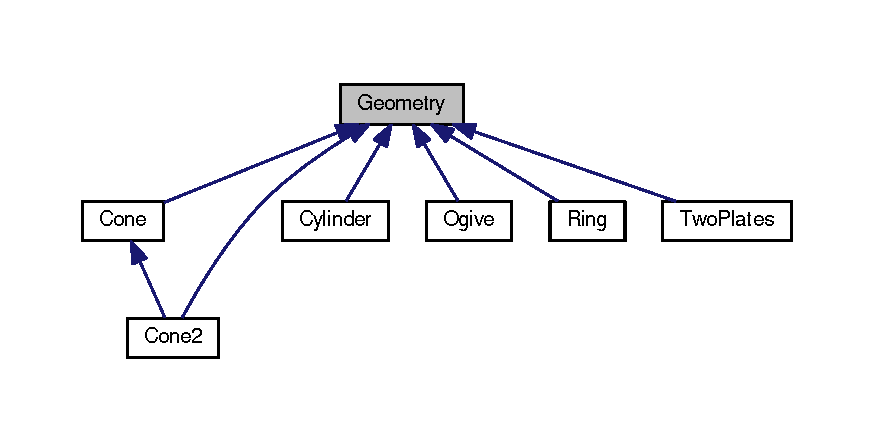
\includegraphics[width=123pt]{classGeometry__inherit__graph}
\end{center}
\end{figure}
\subsection*{Public Member Functions}
\begin{CompactItemize}
\item 
\hypertarget{classGeometry_9f0fe2c1f7e8a6b0d6454f5065b4e606}{
\textbf{Geometry} (std::string, int)}
\label{classGeometry_9f0fe2c1f7e8a6b0d6454f5065b4e606}

\item 
\hypertarget{classGeometry_ee462b9ebbf2e943f8199d5ee8facc8c}{
virtual void \textbf{computeEnergy} (double, std::vector$<$ \hyperlink{classParticle}{Particle} $\ast$ $>$ \&)=0}
\label{classGeometry_ee462b9ebbf2e943f8199d5ee8facc8c}

\item 
\hypertarget{classGeometry_63a40c7e8ca800baa0203850bc96b295}{
virtual void \textbf{computeIncrements} ()}
\label{classGeometry_63a40c7e8ca800baa0203850bc96b295}

\item 
\hypertarget{classGeometry_ab2d4db916d7c8541af6624a82b2d4df}{
virtual void \textbf{setSections} (double)=0}
\label{classGeometry_ab2d4db916d7c8541af6624a82b2d4df}

\item 
\hypertarget{classGeometry_3e77ac889d1e440c24efbde630aa1933}{
virtual void \textbf{computeGeometry} ()=0}
\label{classGeometry_3e77ac889d1e440c24efbde630aa1933}

\item 
\hypertarget{classGeometry_8ba01f4e4d4c0bf0860eb948c6567642}{
virtual void \textbf{computeNodalEnergy} ()}
\label{classGeometry_8ba01f4e4d4c0bf0860eb948c6567642}

\item 
\hypertarget{classGeometry_340099102a94c6fcecd1b9a4f34f9d1e}{
virtual void \textbf{computeNodalPower} ()}
\label{classGeometry_340099102a94c6fcecd1b9a4f34f9d1e}

\item 
\hypertarget{classGeometry_f5fa359d8794cc8d54e0aeafdd3a50e3}{
virtual void \textbf{computeNodalPower} (std::vector$<$ double $>$ \&)}
\label{classGeometry_f5fa359d8794cc8d54e0aeafdd3a50e3}

\item 
\hypertarget{classGeometry_4f2e62b82b91402b4f9c8fbf26048974}{
void \textbf{drawGeometry} ()}
\label{classGeometry_4f2e62b82b91402b4f9c8fbf26048974}

\item 
\hypertarget{classGeometry_c19e292e9134717046f74f60ec1f8a97}{
void \textbf{drawScalar} ()}
\label{classGeometry_c19e292e9134717046f74f60ec1f8a97}

\item 
\hypertarget{classGeometry_e9a734546513a78cbf653ed190f5b6df}{
virtual void \textbf{outputEnergyFile} ()=0}
\label{classGeometry_e9a734546513a78cbf653ed190f5b6df}

\item 
\hypertarget{classGeometry_b01547dec4f04ba548f85f1b2ca4cebf}{
virtual void \textbf{outputPowerFile} ()=0}
\label{classGeometry_b01547dec4f04ba548f85f1b2ca4cebf}

\item 
\hypertarget{classGeometry_60e1424a222ba59284b81812aff34148}{
virtual void \textbf{outputTable} ()=0}
\label{classGeometry_60e1424a222ba59284b81812aff34148}

\item 
\hypertarget{classGeometry_565f5b7736c4b0894732900199903d54}{
std::string \textbf{getType} ()}
\label{classGeometry_565f5b7736c4b0894732900199903d54}

\end{CompactItemize}
\subsection*{Protected Attributes}
\begin{CompactItemize}
\item 
\hypertarget{classGeometry_734ed6644e4e3b98f157e6707c30069a}{
std::string \textbf{type}}
\label{classGeometry_734ed6644e4e3b98f157e6707c30069a}

\item 
\hypertarget{classGeometry_0efc4bf9252077abca96c1c198eefa33}{
int \textbf{sections}}
\label{classGeometry_0efc4bf9252077abca96c1c198eefa33}

\item 
\hypertarget{classGeometry_5e34644bfae4c1df92cb6bf98a8c62c7}{
int \textbf{sectors}}
\label{classGeometry_5e34644bfae4c1df92cb6bf98a8c62c7}

\item 
\hypertarget{classGeometry_1a43a92c349f4ce1f2dc2438bd6cbe1e}{
double \textbf{slope}}
\label{classGeometry_1a43a92c349f4ce1f2dc2438bd6cbe1e}

\item 
\hypertarget{classGeometry_89deb9b2585c4f7b1f47c6568e78ba54}{
std::map$<$ double, std::vector$<$ double $>$ $>$ \textbf{energies}}
\label{classGeometry_89deb9b2585c4f7b1f47c6568e78ba54}

\item 
\hypertarget{classGeometry_6babe7f0fe2ceaf892042432c75c17ca}{
std::map$<$ double, std::vector$<$ double $>$ $>$ \textbf{powers}}
\label{classGeometry_6babe7f0fe2ceaf892042432c75c17ca}

\item 
\hypertarget{classGeometry_9f5642ca54e0353b871d733e25ccc56e}{
std::map$<$ int, \hyperlink{classNode}{Node} $\ast$ $>$ \textbf{nodes}}
\label{classGeometry_9f5642ca54e0353b871d733e25ccc56e}

\item 
\hypertarget{classGeometry_cef6e83971679a9c4672c3b610acb58e}{
std::vector$<$ \hyperlink{classElement}{Element} $\ast$ $>$ \textbf{elements}}
\label{classGeometry_cef6e83971679a9c4672c3b610acb58e}

\item 
\hypertarget{classGeometry_ed9f7f434ae099a62be5c20f9915be90}{
std::string \textbf{plotTitle}}
\label{classGeometry_ed9f7f434ae099a62be5c20f9915be90}

\item 
\hypertarget{classGeometry_ed47a80e867e618e98272e830d297deb}{
vtkPoints $\ast$ \textbf{gridPoints}}
\label{classGeometry_ed47a80e867e618e98272e830d297deb}

\item 
\hypertarget{classGeometry_49e66de69aa22b88759e903e1ae06c9b}{
vtkFloatArray $\ast$ \textbf{scalar}}
\label{classGeometry_49e66de69aa22b88759e903e1ae06c9b}

\item 
\hypertarget{classGeometry_ebabda9f0c07ecb986195857913b4ee8}{
vtkUnstructuredGrid $\ast$ \textbf{grid}}
\label{classGeometry_ebabda9f0c07ecb986195857913b4ee8}

\item 
\hypertarget{classGeometry_22b4feeba28c4834bc9ac42e838cb7bb}{
vtkRenderWindow $\ast$ \textbf{renWin}}
\label{classGeometry_22b4feeba28c4834bc9ac42e838cb7bb}

\item 
\hypertarget{classGeometry_994d1c4d7c8ce0622fcf7a96b5d234af}{
vtkInteractorStyleTrackballCamera $\ast$ \textbf{style}}
\label{classGeometry_994d1c4d7c8ce0622fcf7a96b5d234af}

\item 
\hypertarget{classGeometry_6563f9a823d1dcee59554a5d093d6c73}{
vtkRenderWindowInteractor $\ast$ \textbf{iren}}
\label{classGeometry_6563f9a823d1dcee59554a5d093d6c73}

\item 
\hypertarget{classGeometry_0893a3a686dc14327816c9648efe8662}{
vtkRenderer $\ast$ \textbf{ren}}
\label{classGeometry_0893a3a686dc14327816c9648efe8662}

\item 
\hypertarget{classGeometry_f314d57676056969da57788a60954926}{
vtkDataSetMapper $\ast$ \textbf{aDataSetMapper}}
\label{classGeometry_f314d57676056969da57788a60954926}

\item 
\hypertarget{classGeometry_86a213e57fee0c578d220d8015c2891b}{
vtkActor $\ast$ \textbf{anActor}}
\label{classGeometry_86a213e57fee0c578d220d8015c2891b}

\item 
\hypertarget{classGeometry_aabe40cbb12206d80e4376367568934b}{
vtkLookupTable $\ast$ \textbf{table}}
\label{classGeometry_aabe40cbb12206d80e4376367568934b}

\item 
\hypertarget{classGeometry_f87eb1e4ab0922d0475afc67061ae30a}{
vtkScalarBarActor $\ast$ \textbf{barActor}}
\label{classGeometry_f87eb1e4ab0922d0475afc67061ae30a}

\item 
\hypertarget{classGeometry_17c7a286dc0a428e8a32db4c8d54bb5e}{
vtkAxesActor $\ast$ \textbf{axes}}
\label{classGeometry_17c7a286dc0a428e8a32db4c8d54bb5e}

\item 
\hypertarget{classGeometry_d611799bc0eb8825c963bd6d56181d8c}{
vtkOrientationMarkerWidget $\ast$ \textbf{widget}}
\label{classGeometry_d611799bc0eb8825c963bd6d56181d8c}

\end{CompactItemize}


\subsection{Detailed Description}
\begin{Desc}
\item[Author:]Daniel Iglesias $<$\href{mailto:daniel.iglesias@ciemat.es}{\tt daniel.iglesias@ciemat.es}$>$ \end{Desc}


The documentation for this class was generated from the following files:\begin{CompactItemize}
\item 
src/\hyperlink{geometry_8h}{geometry.h}\item 
src/geometry.cpp\end{CompactItemize}

\hypertarget{classNode}{\section{Node Class Reference}
\label{classNode}\index{Node@{Node}}
}


{\ttfamily \#include $<$/home/daniel.\-iglesias/\-Projects/\-Heat\-Surf/src/node.\-h$>$}

\subsection*{Public Member Functions}
\begin{DoxyCompactItemize}
\item 
\hyperlink{classNode_ad7a34779cad45d997bfd6d3d8043c75f}{Node} ()
\item 
\hyperlink{classNode_ab67eabb0fef1465a1d7d1e11997ddd4d}{Node} (double, double, double)
\item 
\hyperlink{classNode_aa0840c3cb5c7159be6d992adecd2097c}{$\sim$\-Node} ()
\item 
void \hyperlink{classNode_a93d1fc91852d3698d94625f0178df03f}{set\-Scalar} (double scalar\-\_\-in)
\item 
void \hyperlink{classNode_aaa144bb5a91e238a24714f9c21e1f691}{add\-Scalar} (double scalar\-\_\-in)
\item 
void \hyperlink{classNode_a30669c547c3613eb296358270fa034fb}{add\-Density3\-D} (double dens\-\_\-in)
\item 
double \hyperlink{classNode_aaa123501583ea9775583c2c46f755c8f}{get\-Scalar} ()
\item 
void \hyperlink{classNode_ad1eeb7e6ca4fc6d627ca6ff662f8e442}{add\-Density} (double density\-\_\-in)
\item 
double \hyperlink{classNode_a586272c977653ba24e1292b4dc42f8c6}{get\-Density} ()
\item 
double \hyperlink{classNode_a8d8ccf6a6da7717ea6aa67e52c7c9017}{get\-X} ()
\item 
double \hyperlink{classNode_a8877121bf44537ccbe2f3c441fa3b664}{get\-Y} ()
\item 
double \hyperlink{classNode_ab26d80e97604621eab868ebacda71304}{get\-Z} ()
\end{DoxyCompactItemize}


\subsection{Detailed Description}
\begin{DoxyAuthor}{Author}
Daniel Iglesias \href{mailto:daniel.iglesias@ciemat.es}{\tt daniel.\-iglesias@ciemat.\-es} 
\end{DoxyAuthor}


\subsection{Constructor \& Destructor Documentation}
\hypertarget{classNode_ad7a34779cad45d997bfd6d3d8043c75f}{\index{Node@{Node}!Node@{Node}}
\index{Node@{Node}!Node@{Node}}
\subsubsection[{Node}]{\setlength{\rightskip}{0pt plus 5cm}Node\-::\-Node (
\begin{DoxyParamCaption}
{}
\end{DoxyParamCaption}
)}}\label{classNode_ad7a34779cad45d997bfd6d3d8043c75f}
\hypertarget{classNode_ab67eabb0fef1465a1d7d1e11997ddd4d}{\index{Node@{Node}!Node@{Node}}
\index{Node@{Node}!Node@{Node}}
\subsubsection[{Node}]{\setlength{\rightskip}{0pt plus 5cm}Node\-::\-Node (
\begin{DoxyParamCaption}
\item[{double}]{x\-\_\-in, }
\item[{double}]{y\-\_\-in, }
\item[{double}]{z\-\_\-in}
\end{DoxyParamCaption}
)}}\label{classNode_ab67eabb0fef1465a1d7d1e11997ddd4d}
\hypertarget{classNode_aa0840c3cb5c7159be6d992adecd2097c}{\index{Node@{Node}!$\sim$\-Node@{$\sim$\-Node}}
\index{$\sim$\-Node@{$\sim$\-Node}!Node@{Node}}
\subsubsection[{$\sim$\-Node}]{\setlength{\rightskip}{0pt plus 5cm}Node\-::$\sim$\-Node (
\begin{DoxyParamCaption}
{}
\end{DoxyParamCaption}
)}}\label{classNode_aa0840c3cb5c7159be6d992adecd2097c}


\subsection{Member Function Documentation}
\hypertarget{classNode_ad1eeb7e6ca4fc6d627ca6ff662f8e442}{\index{Node@{Node}!add\-Density@{add\-Density}}
\index{add\-Density@{add\-Density}!Node@{Node}}
\subsubsection[{add\-Density}]{\setlength{\rightskip}{0pt plus 5cm}void Node\-::add\-Density (
\begin{DoxyParamCaption}
\item[{double}]{density\-\_\-in}
\end{DoxyParamCaption}
)\hspace{0.3cm}{\ttfamily [inline]}}}\label{classNode_ad1eeb7e6ca4fc6d627ca6ff662f8e442}
\hypertarget{classNode_a30669c547c3613eb296358270fa034fb}{\index{Node@{Node}!add\-Density3\-D@{add\-Density3\-D}}
\index{add\-Density3\-D@{add\-Density3\-D}!Node@{Node}}
\subsubsection[{add\-Density3\-D}]{\setlength{\rightskip}{0pt plus 5cm}void Node\-::add\-Density3\-D (
\begin{DoxyParamCaption}
\item[{double}]{dens\-\_\-in}
\end{DoxyParamCaption}
)\hspace{0.3cm}{\ttfamily [inline]}}}\label{classNode_a30669c547c3613eb296358270fa034fb}
\hypertarget{classNode_aaa144bb5a91e238a24714f9c21e1f691}{\index{Node@{Node}!add\-Scalar@{add\-Scalar}}
\index{add\-Scalar@{add\-Scalar}!Node@{Node}}
\subsubsection[{add\-Scalar}]{\setlength{\rightskip}{0pt plus 5cm}void Node\-::add\-Scalar (
\begin{DoxyParamCaption}
\item[{double}]{scalar\-\_\-in}
\end{DoxyParamCaption}
)\hspace{0.3cm}{\ttfamily [inline]}}}\label{classNode_aaa144bb5a91e238a24714f9c21e1f691}
\hypertarget{classNode_a586272c977653ba24e1292b4dc42f8c6}{\index{Node@{Node}!get\-Density@{get\-Density}}
\index{get\-Density@{get\-Density}!Node@{Node}}
\subsubsection[{get\-Density}]{\setlength{\rightskip}{0pt plus 5cm}double Node\-::get\-Density (
\begin{DoxyParamCaption}
{}
\end{DoxyParamCaption}
)\hspace{0.3cm}{\ttfamily [inline]}}}\label{classNode_a586272c977653ba24e1292b4dc42f8c6}
\hypertarget{classNode_aaa123501583ea9775583c2c46f755c8f}{\index{Node@{Node}!get\-Scalar@{get\-Scalar}}
\index{get\-Scalar@{get\-Scalar}!Node@{Node}}
\subsubsection[{get\-Scalar}]{\setlength{\rightskip}{0pt plus 5cm}double Node\-::get\-Scalar (
\begin{DoxyParamCaption}
{}
\end{DoxyParamCaption}
)\hspace{0.3cm}{\ttfamily [inline]}}}\label{classNode_aaa123501583ea9775583c2c46f755c8f}
\hypertarget{classNode_a8d8ccf6a6da7717ea6aa67e52c7c9017}{\index{Node@{Node}!get\-X@{get\-X}}
\index{get\-X@{get\-X}!Node@{Node}}
\subsubsection[{get\-X}]{\setlength{\rightskip}{0pt plus 5cm}double Node\-::get\-X (
\begin{DoxyParamCaption}
{}
\end{DoxyParamCaption}
)\hspace{0.3cm}{\ttfamily [inline]}}}\label{classNode_a8d8ccf6a6da7717ea6aa67e52c7c9017}
\hypertarget{classNode_a8877121bf44537ccbe2f3c441fa3b664}{\index{Node@{Node}!get\-Y@{get\-Y}}
\index{get\-Y@{get\-Y}!Node@{Node}}
\subsubsection[{get\-Y}]{\setlength{\rightskip}{0pt plus 5cm}double Node\-::get\-Y (
\begin{DoxyParamCaption}
{}
\end{DoxyParamCaption}
)\hspace{0.3cm}{\ttfamily [inline]}}}\label{classNode_a8877121bf44537ccbe2f3c441fa3b664}
\hypertarget{classNode_ab26d80e97604621eab868ebacda71304}{\index{Node@{Node}!get\-Z@{get\-Z}}
\index{get\-Z@{get\-Z}!Node@{Node}}
\subsubsection[{get\-Z}]{\setlength{\rightskip}{0pt plus 5cm}double Node\-::get\-Z (
\begin{DoxyParamCaption}
{}
\end{DoxyParamCaption}
)\hspace{0.3cm}{\ttfamily [inline]}}}\label{classNode_ab26d80e97604621eab868ebacda71304}
\hypertarget{classNode_a93d1fc91852d3698d94625f0178df03f}{\index{Node@{Node}!set\-Scalar@{set\-Scalar}}
\index{set\-Scalar@{set\-Scalar}!Node@{Node}}
\subsubsection[{set\-Scalar}]{\setlength{\rightskip}{0pt plus 5cm}void Node\-::set\-Scalar (
\begin{DoxyParamCaption}
\item[{double}]{scalar\-\_\-in}
\end{DoxyParamCaption}
)\hspace{0.3cm}{\ttfamily [inline]}}}\label{classNode_a93d1fc91852d3698d94625f0178df03f}


The documentation for this class was generated from the following files\-:\begin{DoxyCompactItemize}
\item 
src/\hyperlink{node_8h}{node.\-h}\item 
src/\hyperlink{node_8cpp}{node.\-cpp}\end{DoxyCompactItemize}

\hypertarget{classParticle}{
\section{Particle Class Reference}
\label{classParticle}\index{Particle@{Particle}}
}
{\tt \#include $<$/home/dani/Programs/beam\_\-dump/src/particle.h$>$}

\subsection*{Public Member Functions}
\begin{CompactItemize}
\item 
\hypertarget{classParticle_601373ac2ae46d32c83fffa45d9a0e6b}{
\textbf{Particle} (double, double, double, double, double, double, double, double, double, double)}
\label{classParticle_601373ac2ae46d32c83fffa45d9a0e6b}

\item 
\hypertarget{classParticle_bf0b2c3e900576254d9e76255dfaf81d}{
double \& \textbf{getX} ()}
\label{classParticle_bf0b2c3e900576254d9e76255dfaf81d}

\item 
\hypertarget{classParticle_0fc4232c919f5b1946c2fa74f7a3a9ed}{
double \& \textbf{getY} ()}
\label{classParticle_0fc4232c919f5b1946c2fa74f7a3a9ed}

\item 
\hypertarget{classParticle_d8d1a1de9b549f2a532a8d9a9f97c8fb}{
double \& \textbf{getEnergy} ()}
\label{classParticle_d8d1a1de9b549f2a532a8d9a9f97c8fb}

\end{CompactItemize}


\subsection{Detailed Description}
\begin{Desc}
\item[Author:]Daniel Iglesias $<$\href{mailto:daniel.iglesias@ciemat.es}{\tt daniel.iglesias@ciemat.es}$>$ \end{Desc}


The documentation for this class was generated from the following files:\begin{CompactItemize}
\item 
src/\hyperlink{particle_8h}{particle.h}\item 
src/particle.cpp\end{CompactItemize}

\hypertarget{classSimulation}{
\section{Simulation Class Reference}
\label{classSimulation}\index{Simulation@{Simulation}}
}
{\tt \#include $<$/home/dani/Programs/beam\_\-dump/src/simulation.h$>$}

\subsection*{Public Member Functions}
\begin{CompactItemize}
\item 
\hypertarget{classSimulation_7da40348e01c14777853a5f9e3f4d0e9}{
void \textbf{read} (char $\ast$)}
\label{classSimulation_7da40348e01c14777853a5f9e3f4d0e9}

\item 
\hypertarget{classSimulation_dd5f5f74f34dc0a7e1fe2578f071fb07}{
void \textbf{compute} ()}
\label{classSimulation_dd5f5f74f34dc0a7e1fe2578f071fb07}

\item 
\hypertarget{classSimulation_d1f0c2b7ad3b17c6bd4899624716ed88}{
void \textbf{output} ()}
\label{classSimulation_d1f0c2b7ad3b17c6bd4899624716ed88}

\end{CompactItemize}


\subsection{Detailed Description}
\begin{Desc}
\item[Author:]Daniel Iglesias $<$\href{mailto:daniel.iglesias@ciemat.es}{\tt daniel.iglesias@ciemat.es}$>$ \end{Desc}


The documentation for this class was generated from the following files:\begin{CompactItemize}
\item 
src/\hyperlink{simulation_8h}{simulation.h}\item 
src/simulation.cpp\end{CompactItemize}

\hypertarget{classTwoPlates}{\section{Two\-Plates Class Reference}
\label{classTwoPlates}\index{Two\-Plates@{Two\-Plates}}
}


{\ttfamily \#include $<$/home/daniel.\-iglesias/\-Projects/\-Heat\-Surf/src/twoplates.\-h$>$}



Inheritance diagram for Two\-Plates\-:\nopagebreak
\begin{figure}[H]
\begin{center}
\leavevmode
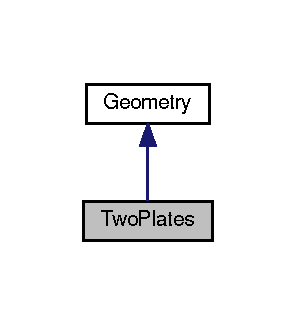
\includegraphics[width=142pt]{classTwoPlates__inherit__graph}
\end{center}
\end{figure}


Collaboration diagram for Two\-Plates\-:\nopagebreak
\begin{figure}[H]
\begin{center}
\leavevmode
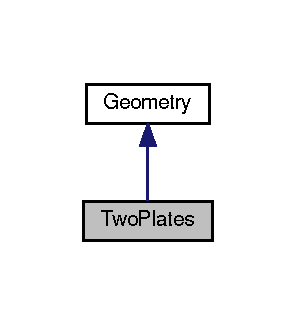
\includegraphics[width=142pt]{classTwoPlates__coll__graph}
\end{center}
\end{figure}
\subsection*{Public Member Functions}
\begin{DoxyCompactItemize}
\item 
\hyperlink{classTwoPlates_a66e45a6d02f3b6026f8dd99ff5d4653e}{Two\-Plates} ()
\item 
\hyperlink{classTwoPlates_ac1dfa39d5a74aad3e53b12c4bbdcff4e}{Two\-Plates} (std\-::string, double, double, int, double, double)
\item 
\hyperlink{classTwoPlates_af74b10840a05812ceb5aa94ceb7a76f6}{$\sim$\-Two\-Plates} ()
\item 
void \hyperlink{classTwoPlates_a23168c87f9097b2c1a4fa8cac4b61049}{set\-Sections} (double)
\item 
void \hyperlink{classTwoPlates_a68c5911a0b3c24f59c3df0335f1e6c94}{compute\-Energy} (double, std\-::vector$<$ \hyperlink{classParticle}{Particle} $\ast$ $>$ \&)
\item 
void \hyperlink{classTwoPlates_a890d6b6ec49ff021d5d34bf1c2a83099}{compute\-Geometry} ()
\item 
void \hyperlink{classTwoPlates_a71bf9bd3453782adb97e94addabe23ec}{residue} (lmx\-::\-Vector$<$ double $>$ \&, lmx\-::\-Vector$<$ double $>$ \&)
\item 
void \hyperlink{classTwoPlates_ad1ae0ed441b0ec1f7650501f648ebfdb}{jacobian} (lmx\-::\-Matrix$<$ double $>$ \&, lmx\-::\-Vector$<$ double $>$ \&)
\item 
void \hyperlink{classTwoPlates_ac0d504d8b9d2cad3b6facd0cb260d7de}{compute\-Intersection} (\hyperlink{classParticle}{Particle} $\ast$)
\item 
void \hyperlink{classTwoPlates_a30eb56de2071f12cb1405057dda35329}{compute\-Nodal\-Power} (\hyperlink{classParticle}{Particle} $\ast$)
\item 
void \hyperlink{classTwoPlates_a8688d978fd1845b370d3fc14d8737e9e}{output\-Table} ()
\item 
void \hyperlink{classTwoPlates_a978c078774fe74e99b8f4064a6126e84}{output\-Power\-File} (int)
\item 
void \hyperlink{classTwoPlates_aec5195987f06df32b1bd1c4c3c0068f9}{output\-Power\-Density\-File} ()
\item 
double \hyperlink{classTwoPlates_a6bff308b65ed2bfe33098ae210626b30}{get\-Length} ()
\end{DoxyCompactItemize}
\subsection*{Additional Inherited Members}


\subsection{Detailed Description}
\begin{DoxyAuthor}{Author}
Daniel Iglesias \href{mailto:daniel.iglesias@ciemat.es}{\tt daniel.\-iglesias@ciemat.\-es} 
\end{DoxyAuthor}


\subsection{Constructor \& Destructor Documentation}
\hypertarget{classTwoPlates_a66e45a6d02f3b6026f8dd99ff5d4653e}{\index{Two\-Plates@{Two\-Plates}!Two\-Plates@{Two\-Plates}}
\index{Two\-Plates@{Two\-Plates}!TwoPlates@{Two\-Plates}}
\subsubsection[{Two\-Plates}]{\setlength{\rightskip}{0pt plus 5cm}Two\-Plates\-::\-Two\-Plates (
\begin{DoxyParamCaption}
{}
\end{DoxyParamCaption}
)}}\label{classTwoPlates_a66e45a6d02f3b6026f8dd99ff5d4653e}
\hypertarget{classTwoPlates_ac1dfa39d5a74aad3e53b12c4bbdcff4e}{\index{Two\-Plates@{Two\-Plates}!Two\-Plates@{Two\-Plates}}
\index{Two\-Plates@{Two\-Plates}!TwoPlates@{Two\-Plates}}
\subsubsection[{Two\-Plates}]{\setlength{\rightskip}{0pt plus 5cm}Two\-Plates\-::\-Two\-Plates (
\begin{DoxyParamCaption}
\item[{std\-::string}]{type\-\_\-in, }
\item[{double}]{par1\-\_\-in, }
\item[{double}]{par2\-\_\-in, }
\item[{int}]{par3\-\_\-in, }
\item[{double}]{width\-\_\-in, }
\item[{double}]{orientation\-\_\-in}
\end{DoxyParamCaption}
)}}\label{classTwoPlates_ac1dfa39d5a74aad3e53b12c4bbdcff4e}


References Geometry\-::length.

\hypertarget{classTwoPlates_af74b10840a05812ceb5aa94ceb7a76f6}{\index{Two\-Plates@{Two\-Plates}!$\sim$\-Two\-Plates@{$\sim$\-Two\-Plates}}
\index{$\sim$\-Two\-Plates@{$\sim$\-Two\-Plates}!TwoPlates@{Two\-Plates}}
\subsubsection[{$\sim$\-Two\-Plates}]{\setlength{\rightskip}{0pt plus 5cm}Two\-Plates\-::$\sim$\-Two\-Plates (
\begin{DoxyParamCaption}
{}
\end{DoxyParamCaption}
)}}\label{classTwoPlates_af74b10840a05812ceb5aa94ceb7a76f6}


\subsection{Member Function Documentation}
\hypertarget{classTwoPlates_a68c5911a0b3c24f59c3df0335f1e6c94}{\index{Two\-Plates@{Two\-Plates}!compute\-Energy@{compute\-Energy}}
\index{compute\-Energy@{compute\-Energy}!TwoPlates@{Two\-Plates}}
\subsubsection[{compute\-Energy}]{\setlength{\rightskip}{0pt plus 5cm}void Two\-Plates\-::compute\-Energy (
\begin{DoxyParamCaption}
\item[{double}]{section, }
\item[{std\-::vector$<$ {\bf Particle} $\ast$ $>$ \&}]{particles}
\end{DoxyParamCaption}
)}}\label{classTwoPlates_a68c5911a0b3c24f59c3df0335f1e6c94}


References Geometry\-::length, Geometry\-::sections, and Geometry\-::sectors.

\hypertarget{classTwoPlates_a890d6b6ec49ff021d5d34bf1c2a83099}{\index{Two\-Plates@{Two\-Plates}!compute\-Geometry@{compute\-Geometry}}
\index{compute\-Geometry@{compute\-Geometry}!TwoPlates@{Two\-Plates}}
\subsubsection[{compute\-Geometry}]{\setlength{\rightskip}{0pt plus 5cm}void Two\-Plates\-::compute\-Geometry (
\begin{DoxyParamCaption}
{}
\end{DoxyParamCaption}
)\hspace{0.3cm}{\ttfamily [virtual]}}}\label{classTwoPlates_a890d6b6ec49ff021d5d34bf1c2a83099}


Implements \hyperlink{classGeometry_a3e77ac889d1e440c24efbde630aa1933}{Geometry}.



References Geometry\-::elements, Geometry\-::grid, Geometry\-::grid\-Points, Geometry\-::length, Geometry\-::nodes, Geometry\-::sections, and Geometry\-::sectors.

\hypertarget{classTwoPlates_ac0d504d8b9d2cad3b6facd0cb260d7de}{\index{Two\-Plates@{Two\-Plates}!compute\-Intersection@{compute\-Intersection}}
\index{compute\-Intersection@{compute\-Intersection}!TwoPlates@{Two\-Plates}}
\subsubsection[{compute\-Intersection}]{\setlength{\rightskip}{0pt plus 5cm}void Two\-Plates\-::compute\-Intersection (
\begin{DoxyParamCaption}
\item[{{\bf Particle} $\ast$}]{particle}
\end{DoxyParamCaption}
)\hspace{0.3cm}{\ttfamily [virtual]}}}\label{classTwoPlates_ac0d504d8b9d2cad3b6facd0cb260d7de}


Implements \hyperlink{classGeometry_ac2e6c74ef25ff3e0c4f46b2c80484881}{Geometry}.



References Particle\-::get\-X(), Particle\-::get\-Xdiv(), Particle\-::get\-Y(), Particle\-::get\-Ydiv(), Particle\-::get\-Z(), Particle\-::get\-Zdiv(), jacobian(), Geometry\-::param\-Trajectories, and residue().

\hypertarget{classTwoPlates_a30eb56de2071f12cb1405057dda35329}{\index{Two\-Plates@{Two\-Plates}!compute\-Nodal\-Power@{compute\-Nodal\-Power}}
\index{compute\-Nodal\-Power@{compute\-Nodal\-Power}!TwoPlates@{Two\-Plates}}
\subsubsection[{compute\-Nodal\-Power}]{\setlength{\rightskip}{0pt plus 5cm}void Two\-Plates\-::compute\-Nodal\-Power (
\begin{DoxyParamCaption}
\item[{{\bf Particle} $\ast$}]{particle}
\end{DoxyParamCaption}
)\hspace{0.3cm}{\ttfamily [virtual]}}}\label{classTwoPlates_a30eb56de2071f12cb1405057dda35329}


Implements \hyperlink{classGeometry_af60650f8ce6d5a220928ccd7395120df}{Geometry}.

\hypertarget{classTwoPlates_a6bff308b65ed2bfe33098ae210626b30}{\index{Two\-Plates@{Two\-Plates}!get\-Length@{get\-Length}}
\index{get\-Length@{get\-Length}!TwoPlates@{Two\-Plates}}
\subsubsection[{get\-Length}]{\setlength{\rightskip}{0pt plus 5cm}double Two\-Plates\-::get\-Length (
\begin{DoxyParamCaption}
{}
\end{DoxyParamCaption}
)\hspace{0.3cm}{\ttfamily [inline]}}}\label{classTwoPlates_a6bff308b65ed2bfe33098ae210626b30}


References Geometry\-::length.

\hypertarget{classTwoPlates_ad1ae0ed441b0ec1f7650501f648ebfdb}{\index{Two\-Plates@{Two\-Plates}!jacobian@{jacobian}}
\index{jacobian@{jacobian}!TwoPlates@{Two\-Plates}}
\subsubsection[{jacobian}]{\setlength{\rightskip}{0pt plus 5cm}void Two\-Plates\-::jacobian (
\begin{DoxyParamCaption}
\item[{lmx\-::\-Matrix$<$ double $>$ \&}]{jac, }
\item[{lmx\-::\-Vector$<$ double $>$ \&}]{conf}
\end{DoxyParamCaption}
)}}\label{classTwoPlates_ad1ae0ed441b0ec1f7650501f648ebfdb}


References Geometry\-::length, and Geometry\-::z0.



Referenced by compute\-Intersection().

\hypertarget{classTwoPlates_aec5195987f06df32b1bd1c4c3c0068f9}{\index{Two\-Plates@{Two\-Plates}!output\-Power\-Density\-File@{output\-Power\-Density\-File}}
\index{output\-Power\-Density\-File@{output\-Power\-Density\-File}!TwoPlates@{Two\-Plates}}
\subsubsection[{output\-Power\-Density\-File}]{\setlength{\rightskip}{0pt plus 5cm}void Two\-Plates\-::output\-Power\-Density\-File (
\begin{DoxyParamCaption}
{}
\end{DoxyParamCaption}
)\hspace{0.3cm}{\ttfamily [virtual]}}}\label{classTwoPlates_aec5195987f06df32b1bd1c4c3c0068f9}


Implements \hyperlink{classGeometry_ad5ea8315df4569915beed2cfbe01fac9}{Geometry}.



References Geometry\-::elements, Geometry\-::nodes, and Geometry\-::sectors.

\hypertarget{classTwoPlates_a978c078774fe74e99b8f4064a6126e84}{\index{Two\-Plates@{Two\-Plates}!output\-Power\-File@{output\-Power\-File}}
\index{output\-Power\-File@{output\-Power\-File}!TwoPlates@{Two\-Plates}}
\subsubsection[{output\-Power\-File}]{\setlength{\rightskip}{0pt plus 5cm}void Two\-Plates\-::output\-Power\-File (
\begin{DoxyParamCaption}
\item[{int}]{particles}
\end{DoxyParamCaption}
)\hspace{0.3cm}{\ttfamily [virtual]}}}\label{classTwoPlates_a978c078774fe74e99b8f4064a6126e84}


Implements \hyperlink{classGeometry_a37f5f2788753e4b8dfcf8de787476d56}{Geometry}.



References Geometry\-::elements, and Geometry\-::sectors.

\hypertarget{classTwoPlates_a8688d978fd1845b370d3fc14d8737e9e}{\index{Two\-Plates@{Two\-Plates}!output\-Table@{output\-Table}}
\index{output\-Table@{output\-Table}!TwoPlates@{Two\-Plates}}
\subsubsection[{output\-Table}]{\setlength{\rightskip}{0pt plus 5cm}void Two\-Plates\-::output\-Table (
\begin{DoxyParamCaption}
{}
\end{DoxyParamCaption}
)\hspace{0.3cm}{\ttfamily [virtual]}}}\label{classTwoPlates_a8688d978fd1845b370d3fc14d8737e9e}


Implements \hyperlink{classGeometry_a60e1424a222ba59284b81812aff34148}{Geometry}.



References Geometry\-::length, Geometry\-::nodes, and Geometry\-::sectors.

\hypertarget{classTwoPlates_a71bf9bd3453782adb97e94addabe23ec}{\index{Two\-Plates@{Two\-Plates}!residue@{residue}}
\index{residue@{residue}!TwoPlates@{Two\-Plates}}
\subsubsection[{residue}]{\setlength{\rightskip}{0pt plus 5cm}void Two\-Plates\-::residue (
\begin{DoxyParamCaption}
\item[{lmx\-::\-Vector$<$ double $>$ \&}]{res, }
\item[{lmx\-::\-Vector$<$ double $>$ \&}]{conf}
\end{DoxyParamCaption}
)}}\label{classTwoPlates_a71bf9bd3453782adb97e94addabe23ec}


References Geometry\-::length, and Geometry\-::z0.



Referenced by compute\-Intersection().

\hypertarget{classTwoPlates_a23168c87f9097b2c1a4fa8cac4b61049}{\index{Two\-Plates@{Two\-Plates}!set\-Sections@{set\-Sections}}
\index{set\-Sections@{set\-Sections}!TwoPlates@{Two\-Plates}}
\subsubsection[{set\-Sections}]{\setlength{\rightskip}{0pt plus 5cm}void Two\-Plates\-::set\-Sections (
\begin{DoxyParamCaption}
\item[{double}]{distance}
\end{DoxyParamCaption}
)\hspace{0.3cm}{\ttfamily [virtual]}}}\label{classTwoPlates_a23168c87f9097b2c1a4fa8cac4b61049}


Implements \hyperlink{classGeometry_aab2d4db916d7c8541af6624a82b2d4df}{Geometry}.



References Geometry\-::length, and Geometry\-::sections.



The documentation for this class was generated from the following files\-:\begin{DoxyCompactItemize}
\item 
src/\hyperlink{twoplates_8h}{twoplates.\-h}\item 
src/\hyperlink{twoplates_8cpp}{twoplates.\-cpp}\end{DoxyCompactItemize}

\chapter{beam\_\-dump File Documentation}
\hypertarget{cone_8h}{\section{src/cone.h File Reference}
\label{cone_8h}\index{src/cone.\-h@{src/cone.\-h}}
}


Pure conical geometry.  


{\ttfamily \#include \char`\"{}geometry.\-h\char`\"{}}\\*
Include dependency graph for cone.\-h\-:
\nopagebreak
\begin{figure}[H]
\begin{center}
\leavevmode
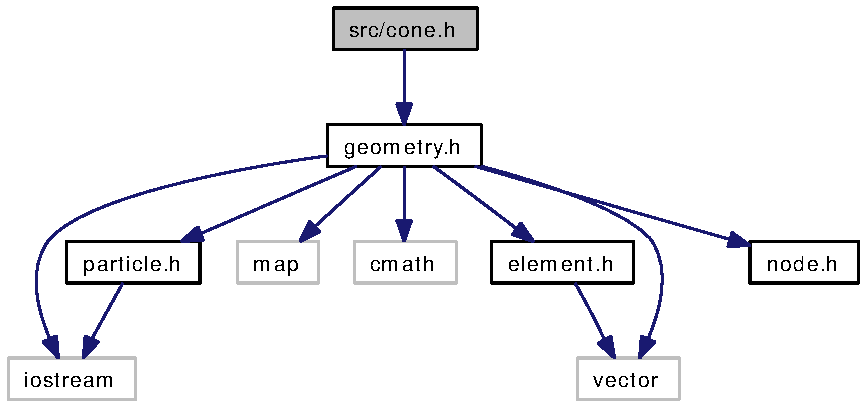
\includegraphics[width=350pt]{cone_8h__incl}
\end{center}
\end{figure}
This graph shows which files directly or indirectly include this file\-:\nopagebreak
\begin{figure}[H]
\begin{center}
\leavevmode
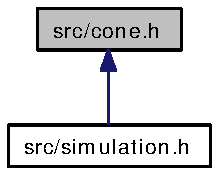
\includegraphics[width=350pt]{cone_8h__dep__incl}
\end{center}
\end{figure}
\subsection*{Classes}
\begin{DoxyCompactItemize}
\item 
class \hyperlink{classCone}{Cone}
\end{DoxyCompactItemize}


\subsection{Detailed Description}
Pure conical geometry. \hyperlink{classGeometry}{Geometry} with origin in s=0 defined by s-\/length and initial diameter (constant slope).

\begin{DoxyAuthor}{Author}
Daniel Iglesias \href{mailto:daniel.iglesias@ciemat.es}{\tt daniel.\-iglesias@ciemat.\-es} 
\end{DoxyAuthor}

\hypertarget{cylinder_8h}{
\section{src/cylinder.h File Reference}
\label{cylinder_8h}\index{src/cylinder.h@{src/cylinder.h}}
}
Pure cylindrical geometry. 

{\tt \#include \char`\"{}geometry.h\char`\"{}}\par


Include dependency graph for cylinder.h:\nopagebreak
\begin{figure}[H]
\begin{center}
\leavevmode
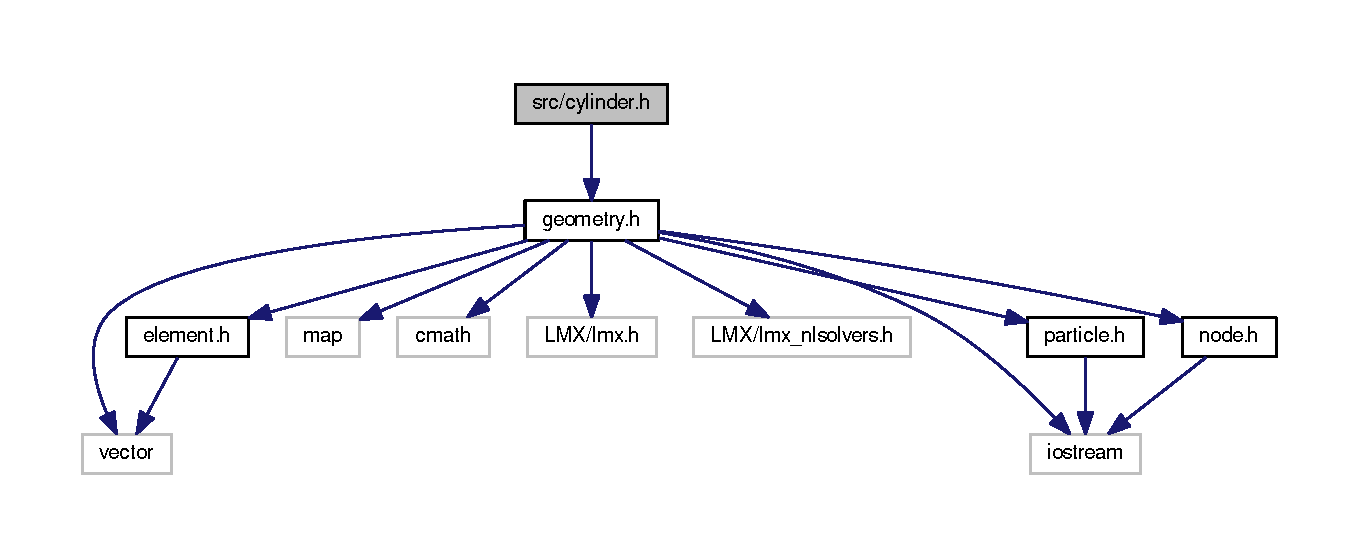
\includegraphics[width=226pt]{cylinder_8h__incl}
\end{center}
\end{figure}


This graph shows which files directly or indirectly include this file:\nopagebreak
\begin{figure}[H]
\begin{center}
\leavevmode
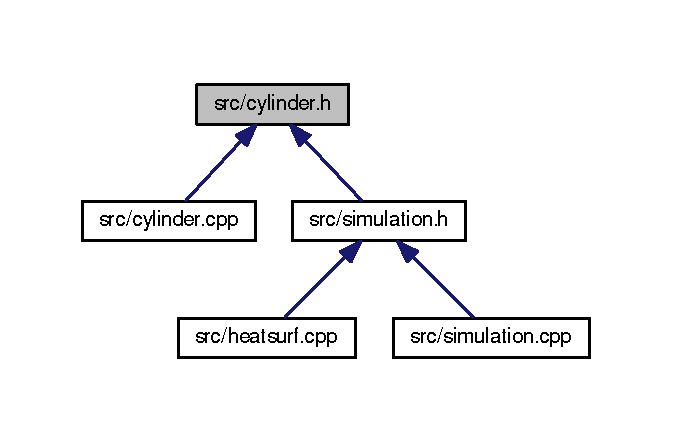
\includegraphics[width=70pt]{cylinder_8h__dep__incl}
\end{center}
\end{figure}
\subsection*{Classes}
\begin{CompactItemize}
\item 
class \hyperlink{classCylinder}{Cylinder}
\end{CompactItemize}


\subsection{Detailed Description}
Pure cylindrical geometry. 

\hyperlink{classGeometry}{Geometry} with origin in s=0 defined by s-length and diameter.

\begin{Desc}
\item[Author:]Daniel Iglesias $<$\href{mailto:daniel.iglesias@ciemat.es}{\tt daniel.iglesias@ciemat.es}$>$ \end{Desc}

\hypertarget{element_8h}{\section{src/element.h File Reference}
\label{element_8h}\index{src/element.\-h@{src/element.\-h}}
}


Facet planar geometry for graphical representation purposes.  


{\ttfamily \#include $<$vector$>$}\\*
Include dependency graph for element.\-h\-:\nopagebreak
\begin{figure}[H]
\begin{center}
\leavevmode
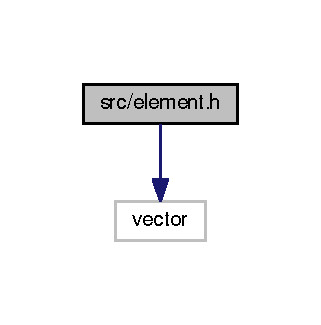
\includegraphics[width=154pt]{element_8h__incl}
\end{center}
\end{figure}
This graph shows which files directly or indirectly include this file\-:\nopagebreak
\begin{figure}[H]
\begin{center}
\leavevmode
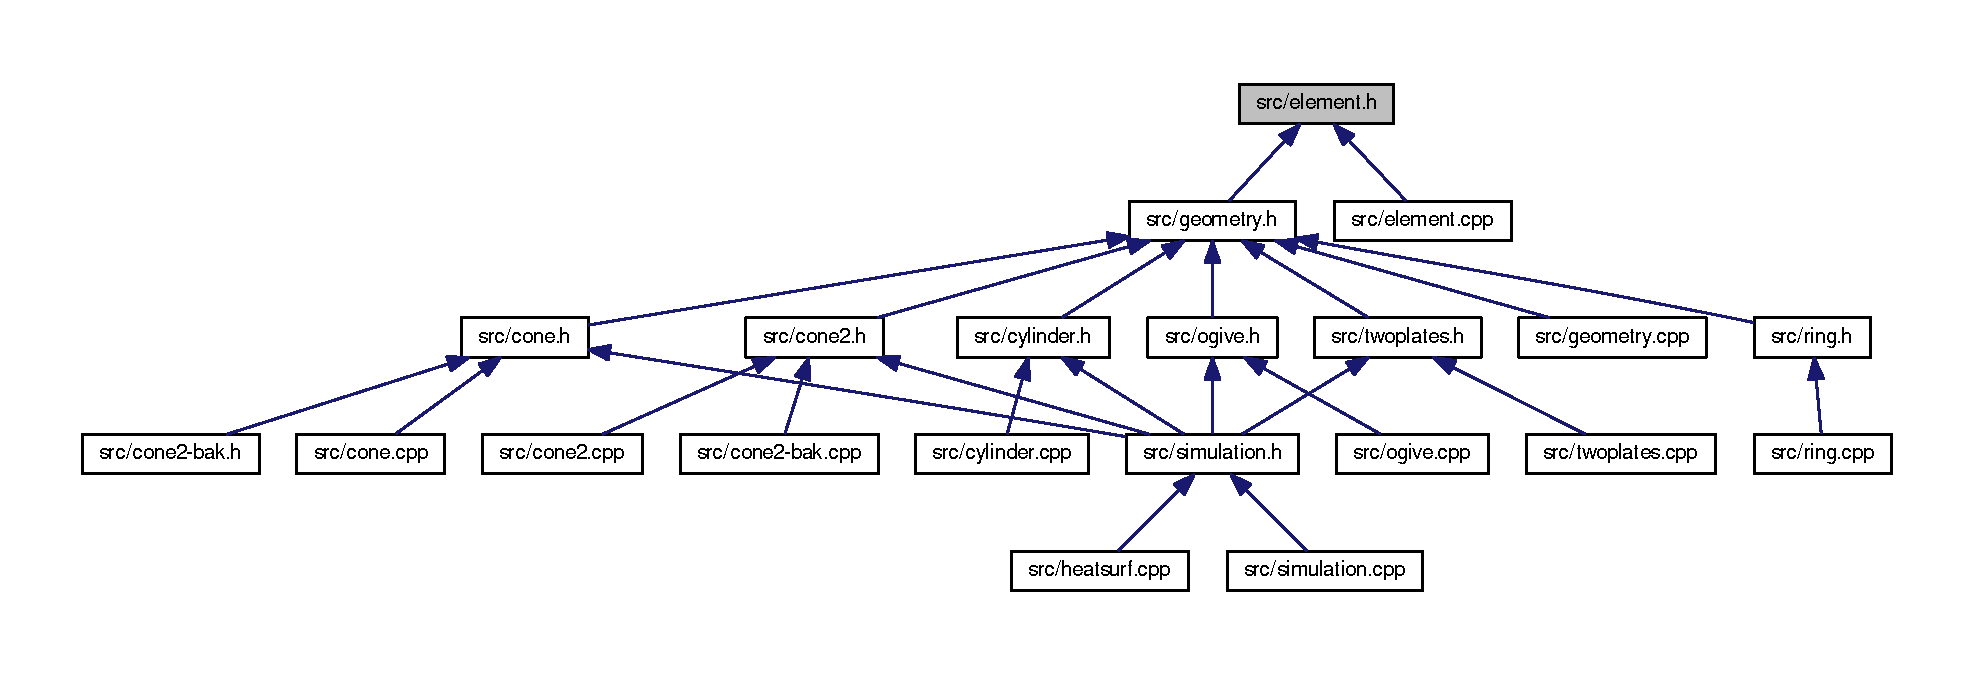
\includegraphics[width=350pt]{element_8h__dep__incl}
\end{center}
\end{figure}
\subsection*{Classes}
\begin{DoxyCompactItemize}
\item 
class \hyperlink{classElement}{Element}
\end{DoxyCompactItemize}


\subsection{Detailed Description}
Facet planar geometry for graphical representation purposes. Uses the \hyperlink{classNode}{Node} class for the defining the vertices. Usually, the dimensions are proportional to the number of sections (longitudinal) and sectors (transversal divisions).

\begin{DoxyAuthor}{Author}
Daniel Iglesias \href{mailto:daniel.iglesias@ciemat.es}{\tt daniel.\-iglesias@ciemat.\-es} 
\end{DoxyAuthor}

\hypertarget{geometry_8h}{
\section{src/geometry.h File Reference}
\label{geometry_8h}\index{src/geometry.h@{src/geometry.h}}
}
Base class for the different geometries. 

{\tt \#include $<$iostream$>$}\par
{\tt \#include $<$vector$>$}\par
{\tt \#include $<$map$>$}\par
{\tt \#include $<$cmath$>$}\par
{\tt \#include \char`\"{}particle.h\char`\"{}}\par
{\tt \#include \char`\"{}element.h\char`\"{}}\par
{\tt \#include \char`\"{}node.h\char`\"{}}\par


Include dependency graph for geometry.h:\nopagebreak
\begin{figure}[H]
\begin{center}
\leavevmode
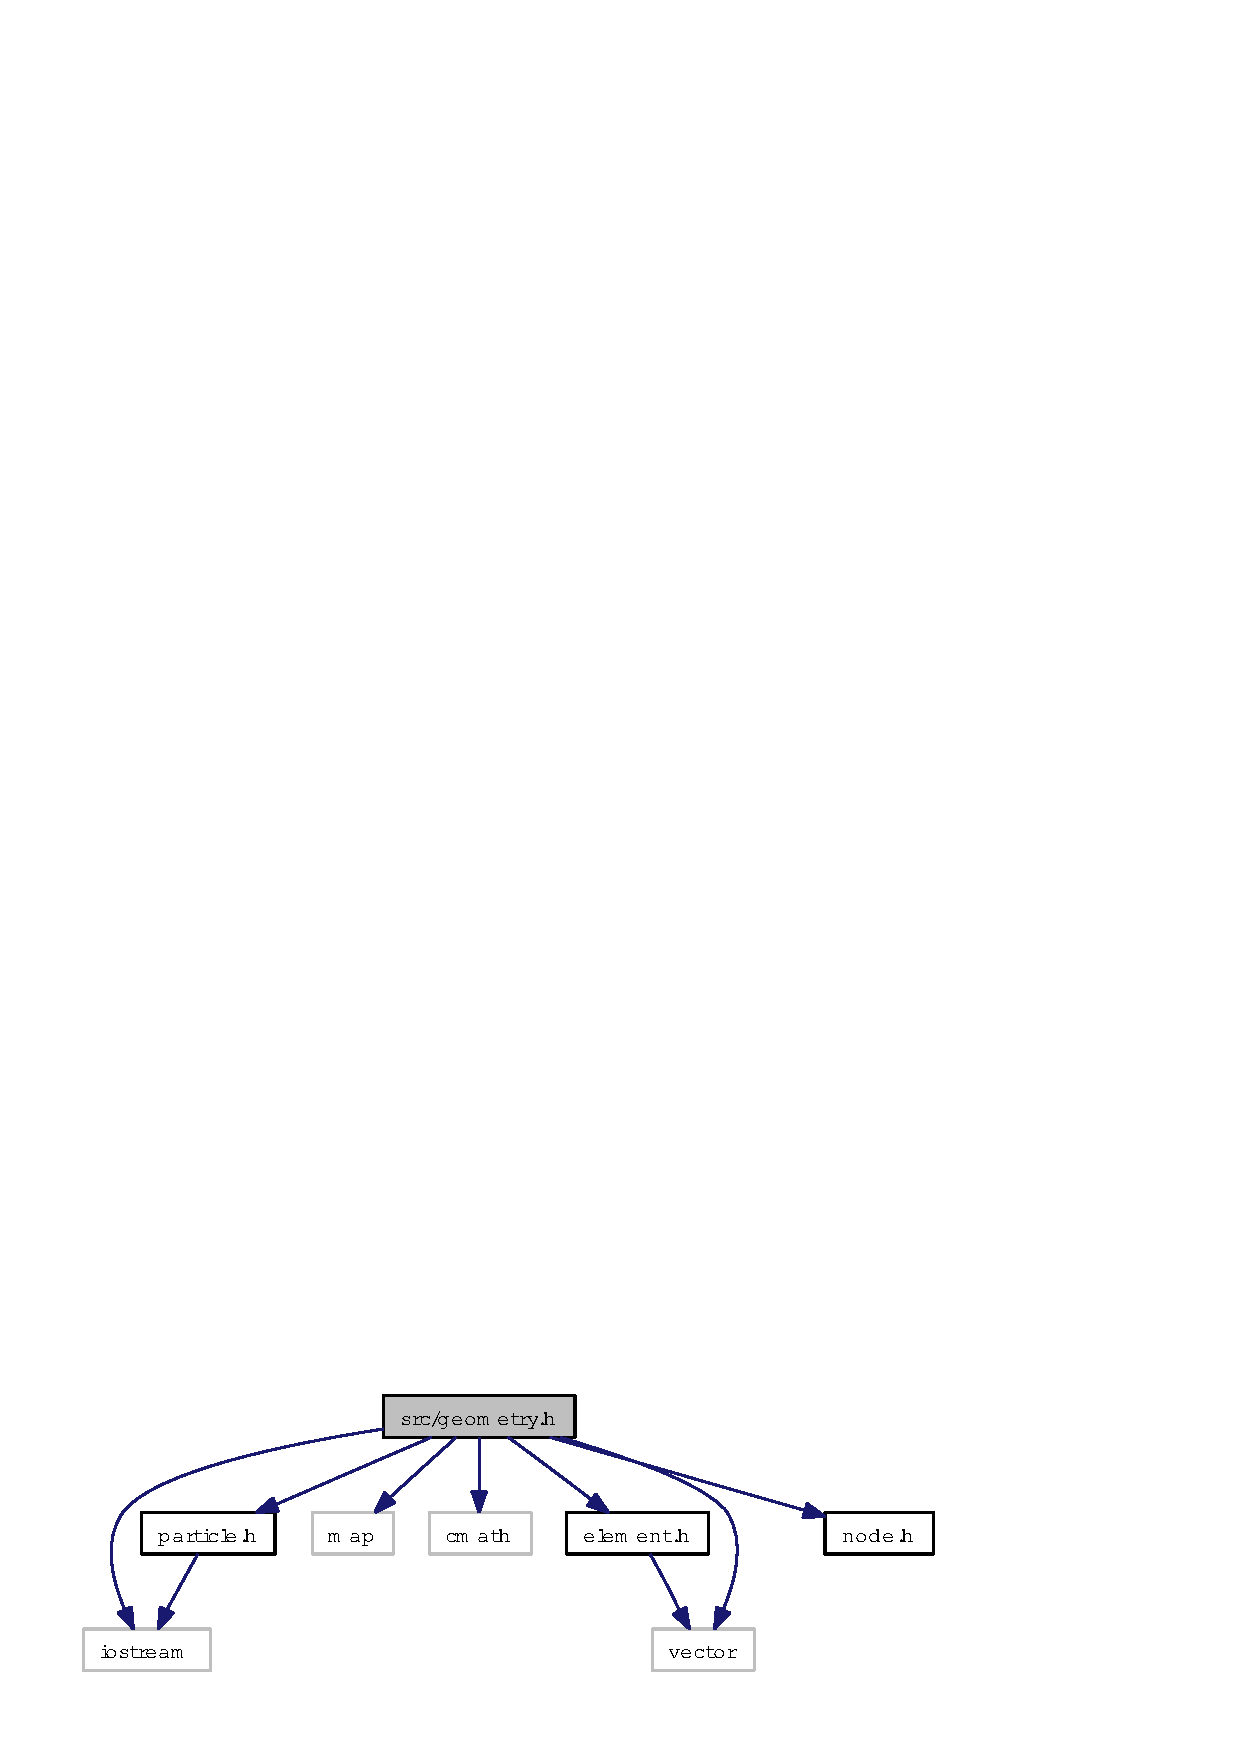
\includegraphics[width=226pt]{geometry_8h__incl}
\end{center}
\end{figure}


This graph shows which files directly or indirectly include this file:\nopagebreak
\begin{figure}[H]
\begin{center}
\leavevmode
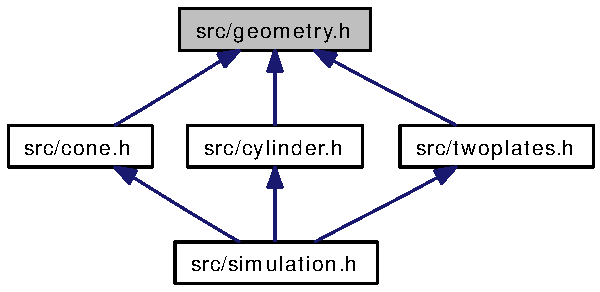
\includegraphics[width=162pt]{geometry_8h__dep__incl}
\end{center}
\end{figure}
\subsection*{Classes}
\begin{CompactItemize}
\item 
class \hyperlink{classGeometry}{Geometry}
\end{CompactItemize}


\subsection{Detailed Description}
Base class for the different geometries. 

Abstract class, cannot be instantiated.

\begin{Desc}
\item[Author:]Daniel Iglesias $<$\href{mailto:daniel.iglesias@ciemat.es}{\tt daniel.iglesias@ciemat.es}$>$ \end{Desc}

\hypertarget{node_8h}{
\section{src/node.h File Reference}
\label{node_8h}\index{src/node.h@{src/node.h}}
}
\hyperlink{classNode}{Node} class for graphical representation purposes. 



This graph shows which files directly or indirectly include this file:\nopagebreak
\begin{figure}[H]
\begin{center}
\leavevmode
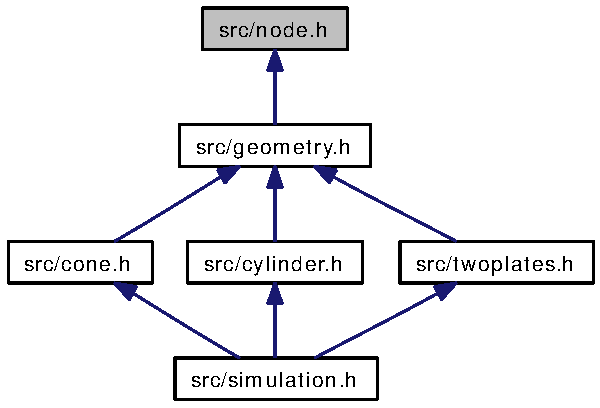
\includegraphics[width=162pt]{node_8h__dep__incl}
\end{center}
\end{figure}
\subsection*{Classes}
\begin{CompactItemize}
\item 
class \hyperlink{classNode}{Node}
\end{CompactItemize}


\subsection{Detailed Description}
\hyperlink{classNode}{Node} class for graphical representation purposes. 

Simple point definition and manipulation. It has a scalar property for storing the power density.

\begin{Desc}
\item[Author:]Daniel Iglesias $<$\href{mailto:daniel.iglesias@ciemat.es}{\tt daniel.iglesias@ciemat.es}$>$ \end{Desc}

\hypertarget{particle_8h}{
\section{src/particle.h File Reference}
\label{particle_8h}\index{src/particle.h@{src/particle.h}}
}
Represents each of the finite charged particles. 

{\tt \#include $<$iostream$>$}\par


Include dependency graph for particle.h:\nopagebreak
\begin{figure}[H]
\begin{center}
\leavevmode
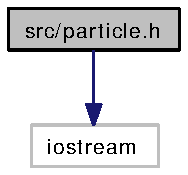
\includegraphics[width=63pt]{particle_8h__incl}
\end{center}
\end{figure}


This graph shows which files directly or indirectly include this file:\nopagebreak
\begin{figure}[H]
\begin{center}
\leavevmode
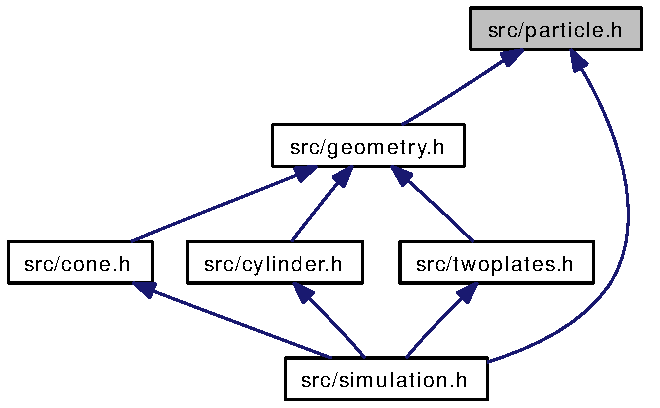
\includegraphics[width=176pt]{particle_8h__dep__incl}
\end{center}
\end{figure}
\subsection*{Classes}
\begin{CompactItemize}
\item 
class \hyperlink{classParticle}{Particle}
\end{CompactItemize}


\subsection{Detailed Description}
Represents each of the finite charged particles. 

Very basic class with stored the x-y position in the plane section and the energy of the particle.

\begin{Desc}
\item[Author:]Daniel Iglesias $<$\href{mailto:daniel.iglesias@ciemat.es}{\tt daniel.iglesias@ciemat.es}$>$ \end{Desc}

\hypertarget{simulation_8h}{
\section{src/simulation.h File Reference}
\label{simulation_8h}\index{src/simulation.h@{src/simulation.h}}
}
Procedures for the program workflow. 

{\tt \#include $<$fstream$>$}\par
{\tt \#include $<$vector$>$}\par
{\tt \#include $<$map$>$}\par
{\tt \#include \char`\"{}cone.h\char`\"{}}\par
{\tt \#include \char`\"{}cylinder.h\char`\"{}}\par
{\tt \#include \char`\"{}twoplates.h\char`\"{}}\par
{\tt \#include \char`\"{}particle.h\char`\"{}}\par


Include dependency graph for simulation.h:\nopagebreak
\begin{figure}[H]
\begin{center}
\leavevmode
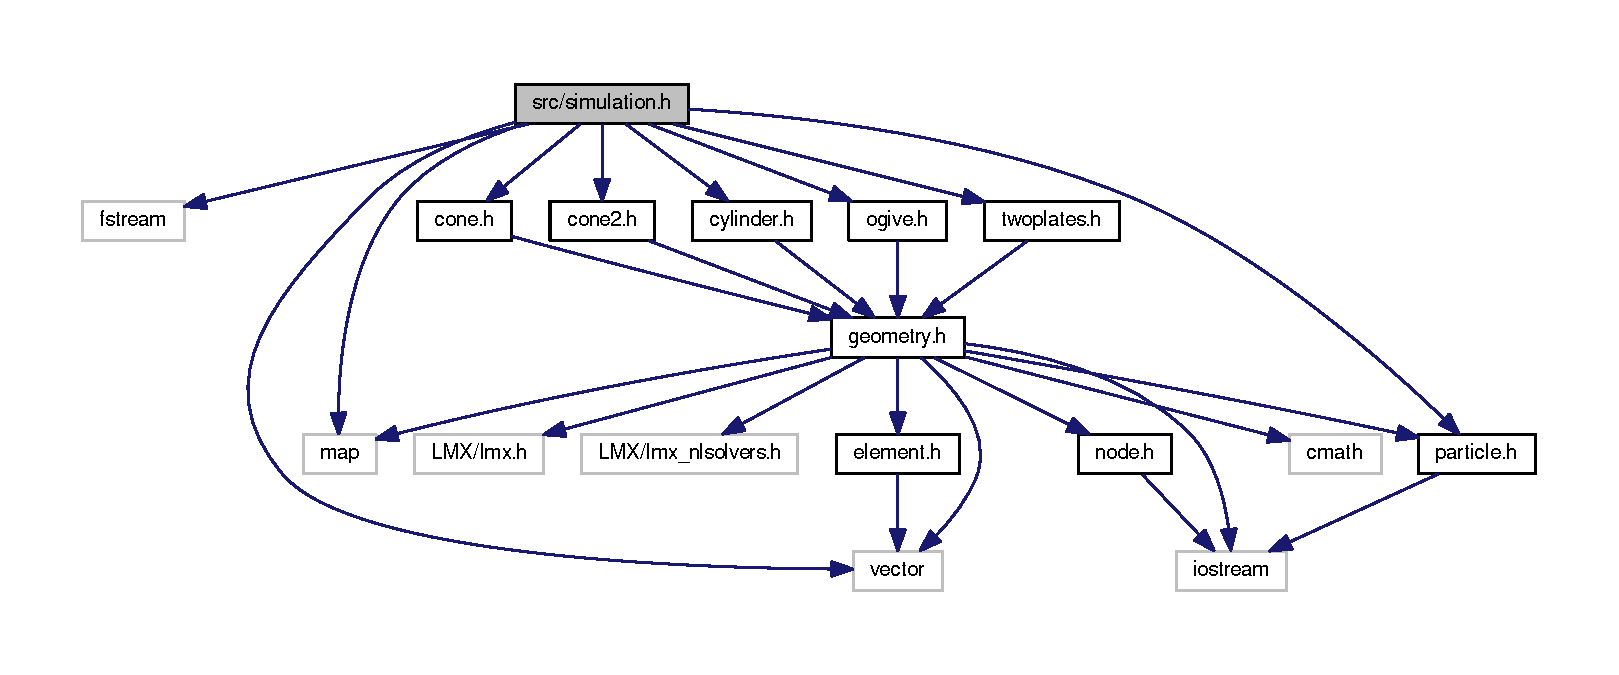
\includegraphics[width=287pt]{simulation_8h__incl}
\end{center}
\end{figure}
\subsection*{Classes}
\begin{CompactItemize}
\item 
class \hyperlink{classSimulation}{Simulation}
\end{CompactItemize}


\subsection{Detailed Description}
Procedures for the program workflow. 

Reads files, creates all of the objects, lauches the computation and creates the output.

\begin{Desc}
\item[Author:]Daniel Iglesias $<$\href{mailto:daniel.iglesias@ciemat.es}{\tt daniel.iglesias@ciemat.es}$>$ \end{Desc}

\hypertarget{twoplates_8h}{\section{src/twoplates.h File Reference}
\label{twoplates_8h}\index{src/twoplates.\-h@{src/twoplates.\-h}}
}


Two symmetrical plates geometry.  


{\ttfamily \#include $<$geometry.\-h$>$}\\*
Include dependency graph for twoplates.\-h\-:
\nopagebreak
\begin{figure}[H]
\begin{center}
\leavevmode
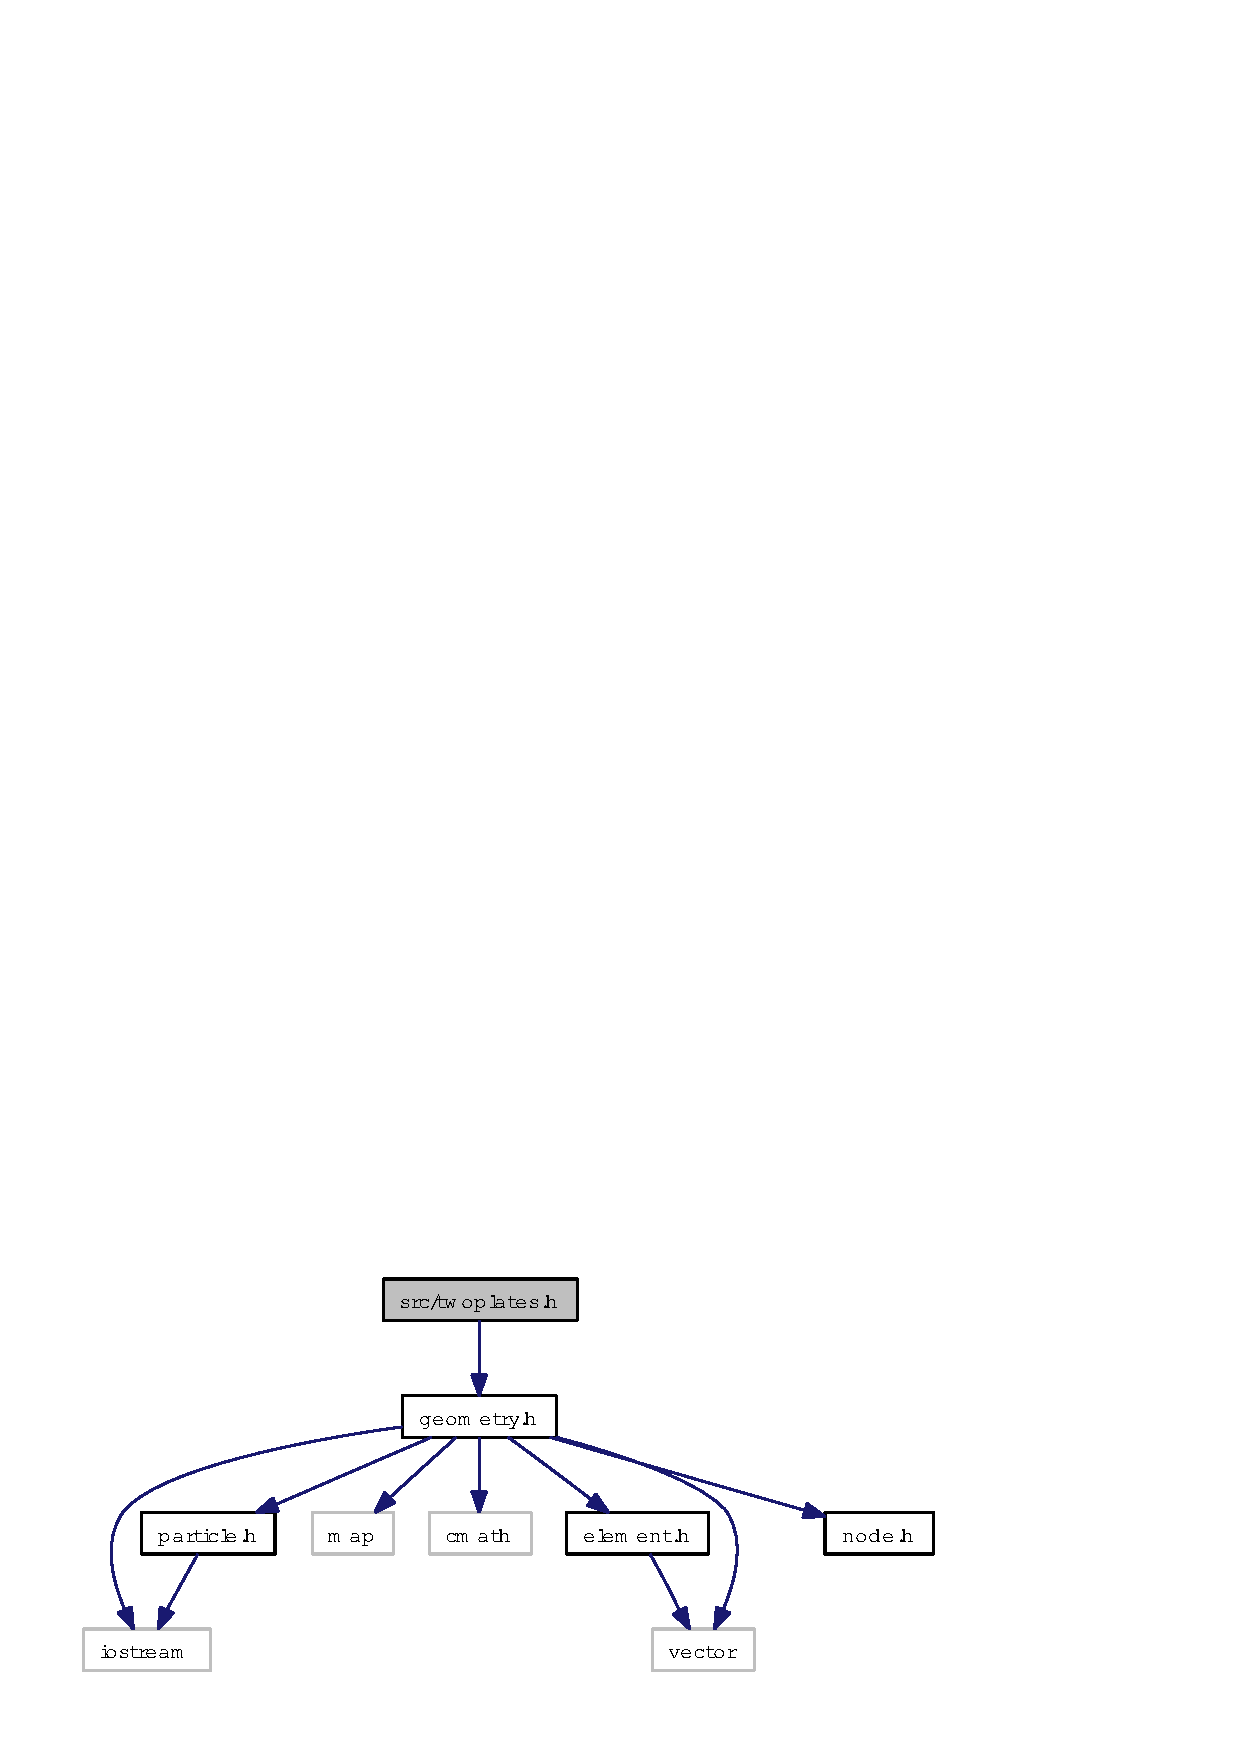
\includegraphics[width=350pt]{twoplates_8h__incl}
\end{center}
\end{figure}
This graph shows which files directly or indirectly include this file\-:\nopagebreak
\begin{figure}[H]
\begin{center}
\leavevmode
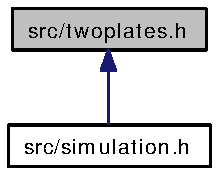
\includegraphics[width=326pt]{twoplates_8h__dep__incl}
\end{center}
\end{figure}
\subsection*{Classes}
\begin{DoxyCompactItemize}
\item 
class \hyperlink{classTwoPlates}{Two\-Plates}
\end{DoxyCompactItemize}


\subsection{Detailed Description}
Two symmetrical plates geometry. \hyperlink{classGeometry}{Geometry} with origin in s=0 defined by s-\/length and initial plate separation (constant slope).

\begin{DoxyAuthor}{Author}
Daniel Iglesias \href{mailto:daniel.iglesias@ciemat.es}{\tt daniel.\-iglesias@ciemat.\-es} 
\end{DoxyAuthor}

\printindex
\end{document}
